\documentclass[notheorems,xcolor=dvipsnames]{beamer}
\usetheme{CambridgeUS}
\useinnertheme{rectangles}
\useoutertheme{infolines}
\usecolortheme[named=Brown]{structure} 

\setbeamercolor{frametitle}{fg=red!90!Brown} %\setbeamercolor{frametitle}{fg=red!255!Brown,bg=Brown!80}
%\setbeamercolor{frametitle}{fg=Brown,bg=Brown!20}
\usepackage{beamerthemeshadow}
\usepackage[utf8]{vietnam}
\usepackage{xcolor,colortbl,color}
\setbeamercovered{dynamic}
\usepackage{setspace} 
%-------------------------------------------------------------------------------
%Sử dụng các gói
\usepackage{etex}
\usepackage{epsfig}
\usepackage{epstopdf}
\usepackage{url}
\usepackage{multirow}
\usepackage[all]{xy}
\usepackage{xspace}
\usepackage{stmaryrd}
\usepackage[ruled,vlined,linesnumbered,resetcount]{algorithm2e}
%----------------------------------------------------------
\usepackage{mdwmath}
\usepackage{mdwtab}
\usepackage{eqparbox}
\usepackage[caption=false,font=footnotesize]{subfig}
\usepackage{fixltx2e}
\usepackage{xcolor}
\usepackage{pgfplots}
\usepackage{tikz}
\usetikzlibrary{shapes}
\usepackage{lipsum}
\usepackage{hyperref}
\usepackage{bookmark}
\usepackage{enumerate}
\usepackage{scrextend}

\usepackage{latexsym}
\usepackage{amssymb}
\usepackage{stmaryrd}
\usepackage{oldgerm} 
\usepackage[english]{babel}
\usepackage[ruled,vlined,linesnumbered]{algorithm2e}
\usepackage{graphicx}
\usepackage{tikz}
\usetikzlibrary{shapes}
\usepackage{algorithmic}
\usepackage{array}
\usepackage{slashbox}
%--------------------------------------------------------------------------
%DEFINE NUMBER FORMAT
%--------------------------------------------------------------------------

%--------------------------------------------------------------------------
%DEFINE ENVIRONMENT
%--------------------------------------------------------------------------

%--------------------------------------------------------------------------
%DEFINE NEW COMMAND
%--------------------------------------------------------------------------

\def\lappr#1#2{#1_{#2^+}}
\def\uappr#1#2{#1_{#2^{\oplus}}}
\def\defeq{\stackrel{\mathrm{def}}{=}}
\def\defequiv{\stackrel{\mathrm{def}}{\equiv}}
\def\implies{\rightarrow}
\def\lneg{\neg}
\def\eqref#1{(\ref{#1})}

%--------------------------------------------------------------
%Dùng cho các ký hiệu
%-------------------------------------------------------------
\newcommand{\mL}		{\mathcal{L}}
\newcommand{\mG}		{\mathcal{G}}
\newcommand{\mA}		{\mathcal{A}}
\newcommand{\mT}		{\mathcal{T}}
\newcommand{\mR}		{\mathcal{R}}
\newcommand{\mI}		{\mathcal{I}}
\newcommand{\mC}		{\mathcal{C}}
\newcommand{\mE}		{\mathcal{E}}
\newcommand{\mP}		{\mathcal{P}}
\newcommand{\mS}		{\mathcal{S}}
\newcommand{\mH}		{\mathcal{H}}
\newcommand{\mO}		{\mathcal{O}}
\newcommand{\mN}		{\mathcal{N}}
\newcommand{\mQ}		{\mathcal{Q}}
\newcommand{\mF}		{\mathcal{F}}
\newcommand{\mU}		{\mathcal{U}}

%\newcommand{\mD}		{\mathbb{D}}
%\newcommand{\mY}		{\mathbb{Y}}
\newcommand{\mbC}		{\mathbb{C}}
\newcommand{\mbD}		{\mathbb{D}}
\newcommand{\mbY}		{\mathbb{Y}}
\newcommand{\mbJ}		{\mathbb{J}}
\newcommand{\mbS}		{\mathbb{S}}

\newcommand{\SigmaI}	{\Sigma_I}
\newcommand{\SigmaA}	{\Sigma_A}
\newcommand{\SigmaC}	{\Sigma_C}
\newcommand{\SigmaR}	{\Sigma_R}
\newcommand{\SigmaDA}	{\Sigma_{dA}}
\newcommand{\SigmaNA}	{\Sigma_{nA}}
\newcommand{\SigmaOR}	{\Sigma_{oR}}
\newcommand{\SigmaDR}	{\Sigma_{dR}}

\newcommand{\SigmaDag}	{\Sigma^\dag}
\newcommand{\SigmaDagI}	{\Sigma^\dag_I}
\newcommand{\SigmaDagA}	{\Sigma^\dag_A}
\newcommand{\SigmaDagC}	{\Sigma^\dag_C}
\newcommand{\SigmaDagR}	{\Sigma^\dag_R}
\newcommand{\SigmaDagDA}{\Sigma^\dag_{dA}}
\newcommand{\SigmaDagNA}{\Sigma^\dag_{nA}}
\newcommand{\SigmaDagOR}{\Sigma^\dag_{oR}}
\newcommand{\SigmaDagDR}{\Sigma^\dag_{dR}}
\newcommand{\PhiDag}	{\Phi^\dag}

\newcommand{\Attrs}		{\mathit{Attrs}}
\newcommand{\True}		{\mathsf{true}}
\newcommand{\False}		{\mathsf{false}}
\newcommand{\Self}		{\mathsf{Self}}
\newcommand{\KB}		{\mathcal{KB}}
\newcommand{\mLS}		{\mL_\Sigma}
\newcommand{\mLSD}		{\mL_{\Sigma^\dag}}
\newcommand{\mLSP}		{\mL_{\Sigma,\Phi}}
\newcommand{\mLSPD}		{\mL_{\Sigma^\dag,\Phi^\dag}}
\newcommand{\SdI}		{{\SigmaDag,\mI}}
\newcommand{\SdPdI}		{{\SigmaDag,\Phi^\dag,\mI}}
\newcommand{\simSdI}	{\sim_{\SigmaDag,\mI}}
\newcommand{\simSdPdI}	{\sim_{\SigmaDag,\Phi^\dag,\mI}}
\newcommand{\LargestContainer}{\mathit{LargestContainer}}

%--------------------------------------------------------------------
\newcommand{\FL}		{$\mathcal{FL}$\xspace}
\newcommand{\FLzero}	{$\mathcal{FL}_0$\xspace}
\newcommand{\FLbot}		{$\mathcal{FL}_\bot$\xspace}
\newcommand{\AL}		{$\mathcal{AL}$\xspace}
\newcommand{\ALC}		{$\mathcal{ALC}$\xspace}
\newcommand{\ALCreg}	{$\mathcal{ALC}_{reg}$\xspace}
\newcommand{\ALN}		{$\mathcal{ALN}$\xspace}
\newcommand{\ALCI}		{$\mathcal{ALCI}$\xspace}
\newcommand{\ALCN}		{$\mathcal{ALCN}$\xspace}
\newcommand{\ALCQ}		{$\mathcal{ALCQ}$\xspace}
\newcommand{\ALCIQ}		{$\mathcal{ALCIQ}$\xspace}
\newcommand{\ALER}		{$\mathcal{ALER}$\xspace}
\newcommand{\LogicS}	{$\mathcal{S}$\xspace}
\newcommand{\SH}		{$\mathcal{SH}$\xspace}
\newcommand{\SI}		{$\mathcal{SI}$\xspace}
\newcommand{\SHI}		{$\mathcal{SHI}$\xspace}
\newcommand{\SHIQ}		{$\mathcal{SHIQ}$\xspace}
\newcommand{\SHIN}		{$\mathcal{SHIN}$\xspace}
\newcommand{\SHIO}		{$\mathcal{SHIO}$\xspace}
\newcommand{\SHOQ}		{$\mathcal{SHOQ}$\xspace}
\newcommand{\SHOIN}		{$\mathcal{SHOIN}$\xspace}
\newcommand{\SHOIQ}		{$\mathcal{SHOIQ}$\xspace}
\newcommand{\SROIQ}		{$\mathcal{SROIQ}$\xspace}

\newcommand{\Ref}			{\mathtt{Ref}}
\newcommand{\Irr}			{\mathtt{Irr}}
\newcommand{\Sym}			{\mathtt{Sym}}
\newcommand{\Tra}			{\mathtt{Tra}}
\newcommand{\Dis}			{\mathtt{Dis}}
\newcommand{\BBCLearn}		{BBCL\xspace}
\newcommand{\dualBBCLearn}	{dual-BBCL\xspace}
\newcommand{\BBCLearnS}		{BBCL2\xspace}

\newcommand{\semiItem}	{\mbox{- }}
\newcommand{\myend}		{\mbox{}\hfill\mbox{{\tiny$\!\blacksquare$}}}
\newcommand{\mdepth}	{\textsf{mdepth}}
\newcommand{\length}	{\textsf{length}}

\newcommand{\tuple}[1]	{\left\langle#1\right\rangle\!}
\newcommand{\ramka}[1]	{\fbox{\parbox{11.3cm}{#1}}}
\newcommand{\mand}		{\sqcap}
\newcommand{\mor}		{\sqcup}
\newcommand{\V}			{\forall}
\newcommand{\E}			{\exists}
\newcommand{\Dom}		{\mathit{dom}}
\newcommand{\Range}		{\mathit{range}}

\newcommand{\PTIME}		{{\sc PTime}\xspace}
\newcommand{\NP}		{{\sc NP}\xspace}
\newcommand{\EXPTIME}	{{\sc ExpTime}\xspace}
\newcommand{\NEXPTIME}	{{\sc NExpTime}\xspace}
\newcommand{\NdEXPTIME}	{{\sc N2ExpTime}\xspace}
\newcommand{\NtEXPTIME}	{{\sc N3ExpTime}\xspace}

%------------------------------------------------------------
%Các ký hiệu cho ví dụ (khái niệm + vai trò)
\newcommand{\Human}			{Human}
\newcommand{\Female}		{Female}
\newcommand{\Male}			{Male}
\newcommand{\Rich}			{Rich}
\newcommand{\Parent}		{Parent}
\newcommand{\Mother}		{Mother}
\newcommand{\Father}		{Father}
\newcommand{\Husband}		{Husband}
\newcommand{\Niece}			{Niece}
\newcommand{\Nephew}		{Nephew}
\newcommand{\Grandfather}	{Grandfather}
\newcommand{\Grandmother}	{Grandmother}
\newcommand{\Grandparent}	{Grandparent}
\newcommand{\BirthYear}		{BirthYear}
\newcommand{\NickName}		{NickName}

\newcommand{\hasChild}		{hasChild}
\newcommand{\hasSon}		{hasSon}
\newcommand{\hasDaughter}	{hasDaughter}
\newcommand{\hasWife}		{hasWife}
\newcommand{\hasHusband}	{hasHusband}
\newcommand{\hasBrother}	{hasBrother}
\newcommand{\hasSister}		{hasSister}
\newcommand{\hasParent}		{hasParent}
\newcommand{\hasSibling}	{hasSibling}
\newcommand{\marriedTo}		{marriedTo}
\newcommand{\hasDescendant}	{hasDescendant}
\newcommand{\hasAscendant}	{hasAscendant}

%Các ký hiệu cho ví dụ (cá thể)
\newcommand{\iLAN}		{\mathsf{LAN}}
\newcommand{\iHUNG}		{\mathsf{HUNG}}
\newcommand{\iHAI}		{\mathsf{HAI}}

\newcommand{\iALICE}	{\mathsf{ALICE}}
\newcommand{\iBOB}		{\mathsf{BOB}}
\newcommand{\iCLAUDIA}	{\mathsf{CLAUDIA}}
\newcommand{\iCALVIN}	{\mathsf{CALVIN}}

\newcommand{\iANH}		{\mathsf{ANH}}
\newcommand{\iPHAP}		{\mathsf{PHAP}}
\newcommand{\iMY}		{\mathsf{MY}}
\newcommand{\iNGA}		{\mathsf{NGA}}
\newcommand{\iTRUNGQUOC}{\mathsf{TRUNGQUOC}}


%-------------------------------------------------------------
\renewcommand{\sharp}		{\#}

%-----------------------------------------------------------------------------
\newcommand{\Publication}{\mathit{Pub}}
\newcommand{\Pub}{\mathit{P}}
\newcommand{\Book}{\mathit{Book}}
\newcommand{\Article}{\mathit{Article}}
\newcommand{\Kind}{\mathit{Kind}}
\newcommand{\Awarded}{\mathit{Awarded}}
\newcommand{\PubName}{\mathit{Title}}
\newcommand{\PubYear}{\mathit{Year}}
\newcommand{\Cites}{\mathit{cites}}
\newcommand{\Citedby}{\mathit{cited\!\_by}}
\newcommand{\UsefulPub}{\mathit{UsefulPub}}
\newcommand{\GoodPub}{\mathit{GoodPub}}
\newcommand{\ExcellentPub}{\mathit{ExcellentPub}}
\newcommand{\RecentPub}{\mathit{RecentPub}}
\newcommand{\CitingP}{\mathit{CitingP}}

\newcommand{\textItL}{\textrm{``Introduction to Logic''}}
\newcommand{\textTEoL}{\textrm{``The Essence of Logic''}}
\newcommand{\textB}{\textrm{``book''}}
\newcommand{\textA}{\textrm{``article''}}
\newcommand{\textC}{\textrm{``conf.~paper''}}

%Định dạng chương, định lý, mệnh đề, ...
%\renewcommand\definitionname{Định nghĩa}
\newtheorem{definition}{Định nghĩa}
\newtheorem{theorem}{Định lý}
\newtheorem{proposition}{Mệnh đề}
\newtheorem{lemma}{Bổ đề}
\newtheorem{corollary}{Hệ quả}
\newtheorem{remark}{Ghi chú}
\newtheorem{example}{Ví dụ}


%-------------------------------------------------------------------------------
%Footer
%-------------------------------------------------------------------------------

\setbeamertemplate{footline}
{
	\leavevmode%
	\hbox{\fontsize{7}{8}\selectfont%
	\begin{beamercolorbox}
		[wd=.20\paperwidth,ht=2.25ex,dp=1ex,right, rightskip=0.6ex]{author in head/foot}%
	    \usebeamerfont{author in head/foot}Trần Thanh Lương
	\end{beamercolorbox}%
	
	\begin{beamercolorbox}
		[wd=.7\paperwidth,ht=2.25ex,dp=1ex,left, leftskip=0.6ex]{title in head/foot}%
		\usebeamerfont{title in head/foot}\insertshorttitle
	\end{beamercolorbox}%
	
	\begin{beamercolorbox}
		[wd=.10\paperwidth,ht=2.25ex,dp=1ex,right]{date in head/foot}%
		\usebeamerfont{date in head/foot}\insertframenumber{}/\inserttotalframenumber\hspace*{1ex}% original: 2ex
	\end{beamercolorbox}}%
}

%--------------------------------------------------------------------------

%--------------------------------------------------------------------------
%DECLARE GENERAL INFORMATION
%--------------------------------------------------------------------------
\title[Học khái niệm đối với các cơ sở tri thức \ldots]{\bf {\normalsize HỌC KHÁI NIỆM ĐỐI VỚI CÁC CƠ SỞ TRI THỨC\\ TRONG LOGIC MÔ TẢ DỰA VÀO MÔ PHỎNG HAI CHIỀU}}
\date{}

\begin{document}

\begin{frame}
	\begin{center}
		{\scriptsize ĐẠI HỌC HUẾ}\\
		{\scriptsize TRƯỜNG ĐẠI HỌC KHOA HỌC}\\[6ex]
		{\bf BÁO CÁO ĐỀ TÀI CẤP CƠ SỞ ĐẠI HỌC HUẾ}
	\end{center}
	\vspace{-3ex}
	\titlepage

	\begin{minipage}{0.4\textwidth}
		\begin{flushleft}
			\emph{\footnotesize Chủ nhiệm đề tài}\\
			{\scriptsize ThS. TRẦN THANH LƯƠNG}
		\end{flushleft}
	\end{minipage}
	\begin{minipage}{0.58\textwidth}
		\begin{flushright}
			\emph{\footnotesize Cán bộ phối hợp thực hiện} \\
			{\scriptsize TS. HOÀNG THỊ LAN GIAO}
		\end{flushright}
	\end{minipage}
\end{frame}

\setstretch{1.15}
%--------------------------------------------------------------------------
\begin{frame}{\bf Nội dung trình bày}
	\begin{enumerate}
		\setlength{\itemsep}{2.0ex}
		\item Giới thiệu tổng quan

		\item Logic mô tả và cơ sở tri thức

		\item Mô phỏng hai chiều trong logic mô tả 
  
		\item Tính bất biến đối với mô phỏng hai chiều

		\item Học khái niệm đối với các cơ sở tri thức trong logic mô tả\\ sử dụng mô phỏng hai chiều
		
		\item Kết luận
\end{enumerate}
\end{frame}
%--------------------------------------------------------------------------

\begin{frame}{\bf Giới thiệu tổng quan}
	\begin{itemize}
		\setlength{\itemsep}{2.0ex}
		\item Logic mô tả có tầm quan trọng đặc biệt $\rightarrow$ cung cấp mô hình lý thuyết cho các hệ thống ngữ nghĩa và ontology.
		
		\item Tìm các khái niệm quan trọng và xây dựng được định nghĩa của các khái niệm đó $\rightarrow$ học khái niệm trong logic mô tả.
		
		\item \textcolor{red}{Học khái niệm trong logic mô tả tương tự như phân lớp nhị phân trong học máy truyền thống}.
		
		\item \textcolor{red}{Điểm khác: các đối tượng không chỉ được đặc tả bằng các thuộc tính mà còn được đặc tả bằng các mối quan hệ giữa các đối tượng}.
		
		\item Các mối quan hệ là một trong những yếu tố làm giàu thêm ngữ nghĩa của hệ thống huấn luyện $\rightarrow$ cần phải tận dụng được chúng như là một lợi thế của các phương pháp học.
	\end{itemize}
\end{frame}
%--------------------------------------------------------------------------

\begin{frame}{\bf Học khái niệm: Ba ngữ cảnh chính}
	\vspace{-1.0ex}
	\begin{block}{}
	{\small 
		\vspace{-1.0ex}
		{\bf Ngữ cảnh 1:} Cho cơ sở tri thức $\KB$ trong logic mô tả $L$ và các tập các cá thể $E^+$, $E^-$. Học khái niệm $C$ trong $L$ sao cho:
		\vspace{-1.0ex}
		\begin{enumerate}
			\setlength{\itemsep}{-0.1ex}
			\item $\KB \models C(a)$ với mọi $a \in E^+$, và
			\item $\KB \models \lnot C(a)$ với mọi $a \in E^-$,
		\end{enumerate}
	}
	\end{block}
	\vspace{-0.7ex}

	\begin{block}{}
	{\small 
		\vspace{-1.0ex}
		{\bf Ngữ cảnh 2:} Ngữ cảnh này khác với ngữ cảnh đã đề cập ở trên là điều kiện thứ~hai được thay bằng một điều kiện yếu hơn:
		\vspace{-1.0ex}
		\begin{enumerate}
			\setlength{\itemsep}{-0.1ex}
			\item $\KB \models C(a)$ với mọi $a \in E^+$, và
			\item $\KB \not\models C(a)$ với mọi $a \in E^-$.
		\end{enumerate}
	}
	\end{block}
	\vspace{-0.7ex}
	
	\begin{block}{}
	{\small 
		\vspace{-1.0ex}
		{\bf Ngữ cảnh 3:} Cho một diễn dịch $\mI$ và các tập các cá thể $E^+$, $E^-$. Học khái niệm $C$ trong logic mô tả $L$ sao cho:
		\vspace{-1.0ex}
		\begin{enumerate}
			\setlength{\itemsep}{-0.1ex}
			\item $\mI \models C(a)$ với mọi $a \in E^+$, và
			\item $\mI \models \lnot C(a)$ với mọi $a \in E^-$.
		\end{enumerate}
		\vspace{-1.0ex}
		Chú ý rằng $\mI \not\models C(a)$ tương đồng với $\mI \models \lnot C(a)$.
	}
	\end{block}
	\vspace{-1.0ex}	
	trong đó, tập $E^+$ chứa các mẫu dương và $E^-$ chứa các mẫu âm của $C$.
\end{frame}

%--------------------------------------------------------------------------
\begin{frame}{\bf Vấn đề đặt ra}
	\begin{block}{}
		{\bf Ngữ cảnh 2:} Cho một diễn dịch $\mI$ và các tập các cá thể $E^+$, $E^-$. Học khái niệm $C$ trong logic mô tả $L$ sao cho:
		\begin{enumerate}
			\setlength{\itemsep}{1.0ex}
			\item $\KB \models C(a)$ với mọi $a \in E^+$, và
			\item $\KB \not\models C(a)$ với mọi $a \in E^-$.
		\end{enumerate}
		trong đó, tập $E^+$ chứa các mẫu dương và $E^-$ chứa các mẫu âm của $C$.
	\end{block}
\end{frame}

%--------------------------------------------------------------------------

\begin{frame}{\bf Mục tiêu chính}
	\begin{enumerate}
		\setlength{\itemsep}{2.0ex}
		\item Nghiên cứu cú pháp, ngữ nghĩa đối với một lớp lớn các logic mô tả. Lớp các logic mô tả này phải có khả năng bao phủ những logic mô tả hữu ích như \SHOIQ, \SROIQ,\,\ldots\; Trên cơ sở đó xây dựng mô phỏng hai chiều cho lớp các logic mô tả này.
			
		\item Xây dựng phương pháp làm mịn phân hoạch miền của các diễn dịch trong logic mô tả dựa trên mô phỏng hai chiều sử dụng các bộ chọn hợp lý cũng như các độ đo về gia lượng thông tin.
		
		\item Đề xuất các thuật toán học khái niệm dựa trên mô phỏng hai chiều cho các cơ sở tri thức trong logic mô tả với ngữ cảnh~(2).
	\end{enumerate}
\end{frame}
%-----------------------------------------------------------------------
%
%\begin{frame}{\bf Cú pháp của \ALC}
%	\begin{block}{\bf Định nghĩa 1.1 (Cú pháp của \ALC)}
%		Cho $\SigmaC$ là tập các {\em tên khái niệm} và $\SigmaR$ là tập các {\em tên vai trò} ($\SigmaC \cap \SigmaR = \emptyset$). Các phần tử của $\SigmaC$ được gọi là {\em khái niệm nguyên tố}. {\em Logic mô tả} \ALC cho phép các khái niệm được định nghĩa một cách đệ quy như sau:
%		\begin{itemize}
%			\item nếu $A \in \SigmaC$ thì $A$ là một khái niệm của \ALC,
%			\item nếu $C$, $D$ là các khái niệm và $r \in \SigmaR$ là một vai trò thì $\top$, $\bot$, $\neg C$, $C \mand D$, $C \mor D$, $\E r.C$ và $\V r.C$ cũng là các khái niệm của \ALC.\myend
%		\end{itemize}
%	\end{block}
%	%
%	\vspace{1.5ex}
%	\noindent
%	Cú pháp của logic mô tả \ALC có thể mô tả bằng các luật sau:
%	\[
%		\begin{array}{r c l}
%			C, D & \longrightarrow&
%			A \mid
%			\top \mid
%			\bot \mid
%			\neg C \mid
%			C\mand D \mid
%			C \mor D \mid
%			\E r.C \mid
%			\V r.C
%		\end{array}
%	\]
%\end{frame}
%%--------------------------------------------------------------------------
%
%\begin{frame}{\bf Ngữ nghĩa của \ALC}
%	\begin{block}{\bf Định nghĩa 1.2 (Ngữ nghĩa của \ALC)}
%	Một {\em diễn dịch} trong logic mô tả \ALC là một bộ \mbox{$\mI = \tuple{\Delta^\mI, \cdot^\mI}$}, trong đó $\Delta^\mI$ là một tập không rỗng được gọi là {\em miền} của $\mI$ và $\cdot^\mI$ là một ánh xạ, được gọi là {\em hàm diễn dịch} của $\mI$, cho phép ánh xạ mỗi cá thể $a \in \SigmaI$ thành một phần tử $a^\mI \in \Delta^\mI$, mỗi tên khái niệm $A \in \SigmaC$ thành một tập $A^\mI \subseteq \Delta^\mI$ và mỗi tên vai trò $r \in \SigmaR$ thành một quan hệ nhị phân $r^\mI \subseteq \Delta^\mI \times \Delta^\mI$.
%	Diễn dịch của các khái niệm phức được xác định như sau:\\[1.0ex]
%	~~~$\top^\mI$ = $\Delta^\mI$, \qquad\qquad\qquad $\bot^\mI$ = $\emptyset$, \qquad\qquad\qquad $(\neg C)^\mI$ = $\Delta^\mI \setminus C^\mI$, \\[0.5ex]
%	~~~$(C \mand D)^\mI$ = $C^\mI \cap D^\mI$, \quad $(C \mor D)^\mI$ = $C^\mI \cup D^\mI$, \\[0.5ex]
%	~~~$(\E r.C)^\mI$ = $\{x \in \Delta^\mI \mid \E y\in \Delta^\mI\; [r^\mI(x,y) \wedge C^\mI(y)]\}$, \\[0.5ex]
%	~~~$(\V r.C)^\mI$ = $\{ x \in \Delta^\mI \mid \V y \in \Delta^\mI\; [r^\mI(x,y) \Rightarrow C^\mI(y)]\}$.\hspace{1.10cm} \myend
%	\end{block}
%\end{frame}
%
%%--------------------------------------------------------------------------
%\begin{frame}{\bf Cú pháp của \ALCreg}
%	\begin{block}{\bf Định nghĩa 1.3 (Cú pháp của \ALCreg)}
%	\label{def:ALCRegSyntax}
%	Cho $\SigmaC$ là tập các {\em tên khái niệm} và $\SigmaR$ là tập các {\em tên vai trò} ($\SigmaC \cap \SigmaR = \emptyset$). Các phần tử của $\SigmaC$ được gọi là {\em khái niệm nguyên tố} và các phần tử của $\SigmaR$ được gọi là {\em vai trò nguyên tố}. {\em Logic mô tả động} \ALCreg cho phép các khái niệm và các vai trò được định nghĩa một cách đệ quy như~sau:
%	\begin{itemize}
%		\item nếu $r \in \SigmaR$ thì $r$ là một vai trò của \ALCreg,
%		\item nếu $A \in \SigmaC$ thì $A$ là một khái niệm của \ALCreg,
%		\item nếu $C$, $D$ là các khái niệm và $R, S$ là các vai trò thì 
%		\begin{itemize}
%			\item $\varepsilon$, $R \circ S$, $R \mor S$, $R^*$, $?C$ là các vai trò của \ALCreg,
%			\item $\top$, $\bot$, $\neg C$, $C \mand D$, $C \mor D$, $\E R.C$ và $\V R.C$ là các khái niệm của~\ALCreg.\myend
%		\end{itemize}
%	\end{itemize}
%	\end{block}
%\end{frame}
%
%%--------------------------------------------------------------------------
%\begin{frame}{\bf Cú pháp và ngữ nghĩa của \ALCreg}
%	Cú pháp \ALCreg có thể mô tả một cách vắn tắt bằng các luật sau:
%	\[
%		\begin{array}{r c l}
%			R, S & \longrightarrow &
%			\varepsilon \mid
%			r \mid 
%			R \circ S \mid
%			R \mor S \mid
%			R^* \mid
%			C?\\[1ex]
%	%
%			C, D & \longrightarrow &
%			A \mid 
%			\top \mid 
%			\bot \mid 
%			\neg C \mid 
%			C \mand D \mid 
%			C \mor D \mid 
%			\E R.C \mid
%			\V R.C
%		\end{array}
%	\]
%	
%	Diễn dịch của các vai trò phức trong \ALCreg được xác định như sau:\\[1.5ex]
%	~~~~~$\varepsilon^\mI = \{\tuple{x,x} \mid x \in \Delta^\mI\}$,\\[1ex]
%	~~~~$(R \circ S)^\mI = R^\mI \circ S^\mI$, \\[1ex]
%	~~~~$(R \mor S)^\mI = R^\mI \cup S^\mI$, \\[1ex]
%	~~~~$(R^*)^\mI = (R^\mI)^*$, \\[1ex]
%	~~~~$(C?)^\mI = \{\tuple{x,x} \mid C^\mI(x)\}$.
%\end{frame}
%--------------------------------------------------------------------------

%\begin{frame}\frametitle{\bf Ngôn ngữ $\mLSP$ và ngữ nghĩa}
%	\begin{itemize}
%		\setlength{\itemsep}{1.7ex}
%		\item {\em Bộ ký tự logic mô tả}: $\Sigma = \SigmaI \cup \SigmaDA \cup \SigmaNA \cup \SigmaOR \cup \SigmaDR$, trong đó:
%		\begin{itemize}
%			\setlength{\itemsep}{1.5ex}
%			\item $\SigmaI$ là tập các {\em cá thể}, 			
%			\item $\SigmaDA$ là tập các {\em thuộc tính rời rạc}, 
%			\item $\SigmaNA$ là tập các {\em thuộc tính số}, 
%			\item $\SigmaOR$ là tập các {\em tên vai trò đối tượng} và 
%			\item $\SigmaDR$ là tập các {\em vai trò dữ liệu}.
%		\end{itemize}
%		\item Đặt $\SigmaA = \SigmaDA \cup \SigmaNA$.
%		\item $A \in \SigmaA$ là thuộc tính Bool nếu $\Range(A) = \{\True,\False\}$, thuộc tính Bool như là các tên khái niệm. 
%		\item Gọi $\SigmaC$ là tập các tên khái niệm của~$\Sigma$.
%	\end{itemize}
%\end{frame}
%
%%--------------------------------------------------------------------------
%\begin{frame}\frametitle{\bf Ngôn ngữ $\mLSP$ và ngữ nghĩa}
%	Các {\em đặc trưng của logic mô tả} gồm:
%	\vspace{0.5ex}
%	\begin{enumerate}
%		\setlength{\itemsep}{1.5ex}
%		\item ~~$\mI$ \qquad {\em vai trò nghịch đảo}, 
%		\item ~~$\mU$ \qquad {\em vai trò phổ quát}  
%		\item ~~$\mO$ \qquad {\em định danh}, 
%		\item ~~$\mF$ \qquad {\em tính chất hàm},
%		\item ~~$\mN$ \qquad {\em hạn chế số lượng không định tính}, 
%		\item ~~$\mQ$ \qquad {\em hạn chế số lượng có định tính},
%		\item ~~$\Self$ \quad\,\!\! {\em tính phản xạ cục bộ của vai trò}.
%	\end{enumerate}
%	\vspace{1.0ex}
%	{\em Tập các đặc trưng của logic mô tả} $\Phi$ một số các đặc trưng trên. 
%	\vspace{1.0ex}
%	
%	$\Phi = \{\mI, \mO, \mQ\}$: nghịch đảo vai trò, định danh, hạn chế số lượng định tính.
%\end{frame}

%--------------------------------------------------------------------------
\begin{frame}\frametitle{}
	\vspace{-1.0ex}
	\begin{block}{\bf Định nghĩa 1.4 (Ngôn ngữ $\mLSP$)}
	\label{def:LSPLanguage}
	\vspace{-1.0ex}
	Cho $\Sigma$ là bộ ký tự logic mô tả, $\Phi$ là tập các đặc trưng của logic mô tả và $\mL$ đại diện cho \ALCreg. Ngôn ngữ logic mô tả $\mLSP$ cho phép các {\em vai trò đối tượng} và các {\em khái niệm} được định nghĩa một cách đệ quy như sau:
	\begin{itemize}
%		\setlength{\itemsep}{1.0ex}
		\item nếu $r \in \SigmaOR$ thì $r$ là một vai trò đối tượng của $\mLSP$,
		\item nếu $A \in \SigmaC$ thì $A$ là một khái niệm của $\mLSP$,
		\item \ldots
		\item nếu $R$ và $S$ là các vai trò đối tượng của $\mLSP$, $C$ và $D$ là các khái niệm của $\mLSP$, $r \in \SigmaOR$, $\sigma \in \SigmaDR$, $a \in \SigmaI$ và $n$ là một số tự nhiên thì
		\begin{itemize}
			\item $\varepsilon$, $R \circ S$ , $R \sqcup S$, $R^*$ và $C?$ là các vai trò đối tượng của $\mLSP$,
			\item $\top$, $\bot$, $\neg C$, $C \mand D$, $C \mor D$, $\E R.C$ và $\V R.C$ là các khái niệm của $\mLSP$,
			\item \ldots
			\item nếu $\Self \in \Phi$ thì $\E r.\Self$ là một khái niệm của $\mLSP$.\myend
		\end{itemize}
	\end{itemize}
	\end{block}
	Xem xét thêm: Thuộc tính, vai trò dữ liệu, tính chất hàm ($\mF$), hạn chế số lượng không định tính ($\mN$).
\end{frame}

%--------------------------------------------------------------------------
%\begin{frame}\frametitle{\bf Ngôn ngữ $\mLSP$ và ngữ nghĩa}
%	\begin{block}{\bf Định nghĩa 1.5 (Ngữ nghĩa của $\mLSP$)}
%		Một {\em diễn dịch} trong $\mLSP$ là một bộ \mbox{$\mI\!=\! \tuple{\Delta^\mI, \cdot^\mI}$}, trong đó $\Delta^\mI$ là một tập không rỗng được gọi là {\em miền} của $\mI$ và $\cdot^\mI$ là một ánh xạ được gọi là {\em hàm diễn dịch} của $\mI$ cho phép ánh xạ mỗi cá thể $a \in \SigmaI$ thành một phần tử $a^\mI \in \Delta^\mI$, mỗi tên khái niệm $A \in \SigmaC$ thành một tập $A^\mI \subseteq \Delta^\mI$, mỗi thuộc tính $A \in \SigmaA \setminus \SigmaC$ thành một hàm từng phần $A^\mI : \Delta^\mI \to \Range(A)$, mỗi tên vai trò đối tượng $r \in \SigmaOR$ thành một quan hệ nhị phân $r^\mI \subseteq \Delta^\mI \times \Delta^\mI$ và mỗi vai trò dữ liệu $\sigma \in \SigmaDR$ thành một quan hệ nhị phân $\sigma^\mI \subseteq \Delta^\mI \times \Range(\sigma)$.
%		
%		Hàm diễn dịch $\cdot^\mI$ được mở rộng cho các vai trò đối tượng phức và các khái niệm phức như trong Hình~1.3, trong đó $\#\Gamma$ ký hiệu cho lực lượng của tập $\Gamma$.\myend
%	\end{block}
%\end{frame}
%%--------------------------------------------------------------------------
%
%\begin{frame}\frametitle{\bf Ngôn ngữ $\mLSP$ và ngữ nghĩa}
%{\scriptsize
%	\begin{figure}[h!]
%		\ramka{
%			\vspace{-2.0ex}
%			\[
%			\begin{array}{c c c}
%			\begin{array}{rcl}
%			(R \circ S)^\mI \!\!\!\!& = &\!\!\!\! R^\mI \circ S^\mI\\[0.5ex]
%			(R \sqcup S)^\mI \!\!\!\!& = &\!\!\!\! R^\mI \cup S^\mI\\[0.5ex]
%			U^\mI \!\!\!\!& = &\!\!\!\!\Delta^\mI \times \Delta^\mI \\[0.5ex]
%			(C \mand D)^\mI \!\!\!\!& = &\!\!\!\! C^\mI \cap D^\mI \\[0.5ex]
%			\end{array} & 
%			\begin{array}{rcl}
%			(R^*)^\mI \!\!\!\!& = &\!\!\!\! (R^\mI)^*\\[0.5ex]
%			(R^-)^\mI \!\!\!\!& = &\!\!\!\! (R^\mI)^{-1} \\[0.5ex]
%			\multicolumn{3}{c}{\top^\mI = \Delta^\mI \qquad \bot^\mI = \emptyset}\\[0.5ex]
%			(C \mor D)^\mI \!\!\!\!& = &\!\!\!\! C^\mI \cup D^\mI \\[0.5ex]    
%			\end{array} & 
%			\begin{array}{rcl}
%			(C?)^\mI \!\!\!\!& = &\!\!\!\! \{ \tuple{x,x} \mid C^\mI(x)\}\\[0.5ex]
%			\varepsilon^\mI \!\!\!\!& = &\!\!\!\! \{\tuple{x,x} \mid x \in \Delta^\mI\}\\[0.5ex]
%			\{a\}^\mI \!\!\!\!& = &\!\!\!\! \{a^\mI\} \\[0.5ex]
%			(\neg C)^\mI \!\!\!\!& = &\!\!\!\! \Delta^\mI \setminus C^\mI \\[0.5ex]
%			\end{array} \\[0.5ex]
%			%  
%			\multicolumn{3}{l}{(A \leq d)^\mI = \{x \in \Delta^\mI \mid A^\mI(x) \textrm{ xác định và } A^\mI(x) \leq d\}} \\[0.5ex]
%			%  
%			\multicolumn{3}{l}{(A \geq d)^\mI = \{x \in \Delta^\mI \mid A^\mI(x) \textrm{ xác định và } A^\mI(x) \geq d \}} \\[0.5ex]
%			%  
%			\multicolumn{3}{l}{(A = d)^\mI = \{x \in \Delta^\mI \mid A^\mI(x) = d\}\qquad\qquad\qquad (A \neq d)^\mI = (\neg (A = d))^\mI} \\[0.5ex]
%			%
%			\multicolumn{3}{l}{(A < d)^\mI = ((A \leq d) \mand (A \neq d))^\mI\ \qquad\qquad\qquad (A > d)^\mI = ((A \geq d) \mand (A \neq d))^\mI} \\[0.5ex]
%			%  
%			\multicolumn{3}{l}{(\V R.C)^\mI = \{ x \in \Delta^\mI \mid \V y\,[R^\mI(x,y) \Rightarrow C^\mI(y)]\}\,\quad (\E r.\Self)^\mI = \{x \in \Delta^\mI \mid r^\mI(x,x)\}} \\[0.5ex]
%			%
%			\multicolumn{3}{l}{(\E R.C)^\mI = \{ x \in \Delta^\mI \mid \E y\,[R^\mI(x,y) \wedge C^\mI(y)]\}\ \; \quad (\E \sigma.\{d\})^\mI = \{ x \in \Delta^\mI \mid \sigma^\mI(x,d)\}} \\[0.5ex]
%			%
%			\multicolumn{3}{l}{(\geq n\,R.C)^\mI = \{x \in \Delta^\mI \mid \#\{y \mid R^\mI(x,y) \wedge C^\mI(y)\} \geq n\} 
%			\qquad (\geq n\,R)^\mI = (\geq n\,R.\top)^\mI} \\[0.5ex]
%			%
%			\multicolumn{3}{l}{(\leq n\,R.C)^\mI = \{x \in \Delta^\mI \mid \#\{y \mid R^\mI(x,y) \wedge C^\mI(y)\} \leq n \}
%			\qquad(\leq n\,R)^\mI = (\leq n\,R.\top)^\mI}
%			\end{array}
%			\vspace{-2.5ex}
%			\]
%		}
%	\end{figure}
%}
%\end{frame}
%--------------------------------------------------------------------------

%\begin{frame}{\bf Diễn dịch trong $\mLSP$}
%	Cho diễn dịch $\mI = \tuple{\Delta^\mI, \cdot^\mI}$ trong ngôn ngữ $\mLSP$. Chúng ta nói rằng đối tượng $x \in \Delta^\mI$ có {\em độ sâu} là $k$ nếu $k$ là số tự nhiên lớn nhất sao cho tồn tại các đối tượng $x_0, x_1, \ldots, x_k \in \Delta^\mI$ khác nhau từng đôi một thỏa mãn:
%	\begin{itemize}
%		\setlength{\itemsep}{2.0ex}
%		\item $x_k = x$ và $x_0 = a^\mI$ với $a \in \SigmaI$,
%		\item $x_i \not= b^\mI$ với mọi $1 \leq i \leq k$ và với mọi $b \in \SigmaI$,
%		\item với mỗi $1 \leq i \leq k$ tồn tại một vai trò đối tượng $R_i$ của $\mLSP$ sao cho $R_i^\mI(x_{i-1}, x_i)$ thỏa~mãn.
%	\end{itemize}
%	
%	\vspace{1.0ex}
%	Chúng ta ký hiệu $\mI_{\mid k}$ là diễn dịch thu được từ diễn dịch $\mI$ bằng cách hạn chế miền $\Delta^\mI$ của diễn dịch $\mI$ chỉ bao gồm tập các đối tượng có độ sâu không lớn hơn $k$ và hàm diễn dịch $\cdot^\mI$ được hạn chế một cách tương ứng.
%\end{frame}

%--------------------------------------------------------------------------
%\begin{frame}\frametitle{\bf Bộ tiên đề vai trò - RBox}
%	\vspace{-1.0ex}
%	\begin{block}{\bf Định nghĩa 1.6 (Tiên đề vai trò)}
%		\label{def:RoleAxiom}
%		\vspace{-1.0ex}
%		Một {\em tiên đề bao hàm vai trò} trong ngôn ngữ $\mLSP$ là một biểu thức có dạng $\varepsilon \sqsubseteq r$ hoặc $R_1 \circ R_2 \circ \cdots \circ R_k \sqsubseteq r$, trong đó $k \geq 1$, $r \in \SigmaOR$ và $R_1, R_2, \ldots,R_k$ là các vai trò đối tượng cơ bản của $\mLSP$ khác với vai trò phổ quát $U$. 
%	%
%		Một {\em khẳng định vai trò} trong ngôn ngữ $\mLSP$ là một biểu thức có dạng $\Ref(r)$, $\Irr(r)$, $\Sym(r)$, $\Tra(r)$ hoặc $\Dis(R, S)$, trong đó $r \in \SigmaOR$ và $R, S$ là các vai trò đối tượng của $\mLSP$ khác với vai trò phổ quát $U$.
%	%
%		Một {\em tiên đề vai trò} trong ngôn ngữ $\mLSP$ là một tiên đề bao hàm vai trò hoặc một khẳng định vai trò trong $\mLSP$.\myend
%	\end{block}
%	
%	\begin{block}{\bf Định nghĩa 1.7 (Bộ tiên đề vai trò)}
%		{\em Bộ tiên đề vai trò} ({\em RBox}) trong ngôn ngữ $\mLSP$ là một tập hữu hạn các tiên đề vai trò trong $\mLSP$.\myend
%	\end{block}
%\end{frame}
%
%%--------------------------------------------------------------------------
%\begin{frame}{\bf Ngữ nghĩa của các tiên đề vai trò}
%	Ngữ nghĩa của các tiên đề vai trò được xác định thông qua diễn dịch $\mI$ như sau:\\[1.5ex]
%	\begin{tabular}{c l c l}
%		& $\mI \models \varepsilon \sqsubseteq r$ & nếu & $\varepsilon^\mI \subseteq r^\mI$,\\[1.5ex]
%		& $\mI \models R_1 \circ R_2 \circ \cdots \circ R_k \sqsubseteq r$ & nếu & $R_1^\mI \circ R_2^\mI \circ \cdots \circ R_k^\mI \sqsubseteq r^\mI$,\\[1.5ex]
%		& $\mI \models \Ref(r)$ & nếu & $r^\mI$ phản xạ,\\[1.5ex]
%		& $\mI \models \Irr(r)$ & nếu & $r^\mI$ không phản xạ,\\[1.5ex]
%		& $\mI \models \Sym(r)$ & nếu & $r^\mI$ đối xứng,\\[1.5ex]
%		& $\mI \models \Tra(r)$ & nếu & $r^\mI$ bắc cầu,\\[1.5ex]
%		& $\mI \models \Dis(R,S)$ & nếu & $R^\mI$ và $S^\mI$ không giao nhau.
%	\end{tabular}
%	\vspace{1.5ex}
%	
%	Giả sử $\varphi$ là một tiên đề vai trò. $\mI$ {\em thỏa mãn} $\varphi$ nếu $\mI \models \varphi$.
%\end{frame}
%%--------------------------------------------------------------------------
%
%\begin{frame}\frametitle{\bf Bộ tiên đề thuật ngữ - TBox}
%	\begin{block}{\bf Định nghĩa 1.8 (Tiên đề thuật ngữ)}
%	\label{def:TerminologyAxiom}
%		Một {\em tiên đề bao hàm khái niệm tổng quát} trong ngôn ngữ $\mLSP$ là một biểu thức có dạng $C \sqsubseteq D$, trong đó $C$ và $D$ là các khái niệm của $\mLSP$. 
%	%
%		Một {\em tiên đề tương đương khái niệm} trong ngôn ngữ $\mLSP$ là một biểu thức có dạng $C \equiv D$, trong đó $C$ và $D$ là các khái niệm của $\mLSP$. 
%	%
%		Một {\em tiên đề thuật ngữ} trong ngôn ngữ $\mLSP$ là một tiên đề bao hàm khái niệm tổng quát hoặc một tiên đề tương đương khái niệm trong $\mLSP$.\myend
%	\end{block}
%	
%	\begin{block}{\bf Định nghĩa 1.9 (Bộ tiên đề thuật ngữ)}
%		{\em Bộ tiên đề thuật ngữ} ({\em TBox}) trong ngôn ngữ $\mLSP$ là một tập hữu hạn các tiên đề thuật ngữ trong $\mLSP$.\myend
%	\end{block}
%\end{frame}
%%--------------------------------------------------------------------------
%
%\begin{frame}{\bf Ngữ nghĩa của các tiên đề thuật ngữ}
%	Đối với tiên đề tương đương khái niệm $C \equiv D$:\\[0.5ex]
%	\begin{itemize}
%		\setlength{\itemsep}{2.0ex}
%		\item Nếu $C$ là một tên khái niệm thì chúng ta nói $C \equiv D$ là một {\em định nghĩa khái niệm} và khái niệm $C$ được gọi là {\em khái niệm định nghĩa}. 
%		\item Một tiên đề tương đương khái niệm $C \equiv D$ có thể được chuyển đổi tương đương thành hai tiên đề bao hàm khái niệm tổng quát là $C \sqsubseteq D$ và $D \sqsubseteq C$.
%	\end{itemize}
%	
%	Ngữ nghĩa của các tiên đề thuật ngữ được xác định thông qua diễn dịch $\mI$ như~sau:\\[1.5ex]
%	\begin{tabular}{c l c l}
%		& $\mI \models C \sqsubseteq D$ & nếu & $C^\mI \subseteq D^\mI$,\\[1.5ex]
%		& $\mI \models C \equiv D$ & nếu & $C^\mI = D^\mI$.
%	\end{tabular}
%	\vspace{1.5ex}
%	
%	Giả sử $\varphi$ là một tiên đề thuật ngữ. $\mI$ {\em thỏa mãn} $\varphi$ nếu $\mI \models \varphi$.
%\end{frame}
%%--------------------------------------------------------------------------
%
%\begin{frame}\frametitle{\bf Bộ khẳng định - ABox}
%	\begin{block}{\bf Định nghĩa 1.10 (Khẳng định cá thể)}
%		\label{def:AssertionIndividual}
%		Một {\em khẳng định cá thể} trong ngôn ngữ $\mLSP$ là một biểu thức có dạng $C(a)$, $R(a,b)$, $\neg R(a,b)$, $a=b$, $a \not=b$, trong đó $C$ là một khái niệm và $R$ là một vai trò đối tượng của $\mLSP$.\myend
%	\end{block}
%	
%	\begin{block}{\bf Định nghĩa 1.11 (Bộ khẳng định cá thể)}
%		\label{def:ABox}
%		{\em Bộ khẳng định cá thể} ({\em ABox}) trong ngôn ngữ $\mLSP$ là một tập hữu hạn các khẳng định cá thể trong $\mLSP$.\myend
%	\end{block}
%\end{frame}
%--------------------------------------------------------------------------

%\begin{frame}{\bf Ngữ nghĩa của khẳng định cá thể}
%	Ngữ nghĩa của các khẳng định cá thể được xác định thông qua diễn dịch $\mI$ như~sau:\\[1.5ex]
%	\begin{tabular}{c l c l}
%		& $\mI \models C(a)$      & nếu & $a^\mI \in C^\mI$, \\[1.5ex] 
%		& $\mI \models R(a,b)$    & nếu & $\tuple{a^\mI,b^\mI} \in R^\mI$,\\[1.5ex]
%		& $\mI \models \neg R(a,b)$ & nếu & $\tuple{a^\mI,b^\mI} \notin R^\mI$.\\[1.5ex]
%		& $\mI \models a = b$     & nếu & $a^\mI = b^\mI$, \\[1.5ex]
%		& $\mI \models a \neq b$  & nếu & $a^\mI \neq b^\mI$.
%	\end{tabular}
%	\vspace{1.5ex}
%	
%	Giả sử $\varphi$ là một khẳng định cá thể. $\mI$ {\em thỏa mãn} $\varphi$ nếu $\mI \models \varphi$.
%\end{frame}

%--------------------------------------------------------------------------
\begin{frame}\frametitle{\bf Cơ sở tri thức và mô hình của cơ sở tri thức}
	\begin{block}{\bf Định nghĩa (Cơ sở tri thức)}
		Một {\em cơ sở tri thức} trong ngôn ngữ $\mLSP$ là một bộ ba \mbox{$\KB = \tuple{\mR, \mT, \mA}$}, trong đó $\mR$ là một RBox, $\mT$ là một TBox và $\mA$ là một ABox trong $\mLSP$.\myend
	\end{block}
	
	\begin{block}{\bf Định nghĩa (Mô hình)}
		Một diễn dịch $\mI$ là một {\em mô hình} của RBox $\mR$ (tương ứng, TBox $\mT$, ABox $\mA$), ký hiệu là $\mI \models \mR$ (tương ứng, $\mI \models \mT$, $\mI \models \mA$), nếu $\mI$ thỏa mãn tất cả các tiên đề vai trò trong $\mR$ (tương ứng, tiên đề thuật ngữ trong $\mT$, khẳng định cá thể trong~$\mA$).
		Một diễn dịch $\mI$ là một {\em mô hình} của cơ sở tri~thức $\KB=\tuple{\mR,\mT, \mA}$, ký hiệu là $\mI \models \KB$, nếu nó là mô hình của cả $\mR$,~$\mT$~và~$\mA$.\myend
	\end{block}
\end{frame}

%%--------------------------------------------------------------------------
%\begin{frame}\frametitle{\bf Cơ sở tri thức và mô hình của cơ sở tri thức}
%	\begin{itemize}
%		\setlength{\itemsep}{1.0ex}
%		\item Một cơ sở tri thức $\KB$ được gọi là {\em thỏa mãn} nếu nó có mô hình. 
%		
%		\item Một cá thể $a$ là {\em thể hiện} của khái niệm $C$ dựa trên $\KB$, ký hiệu là $\KB \models C(a)$, nếu với mọi diễn dịch $\mI$ là mô hình của $\KB$ thì $a^\mI \in C^\mI$. 
%		
%		\item Cá thể $a$ không phải thể hiện của khái niệm $C$ dựa trên $\KB$ được ký hiệu là $\KB \not \models C(a)$.
%		
%		\item Khái niệm $D$ được gọi là {\em bao hàm} khái niệm $C$ dựa trên $\KB$, ký hiệu là $\KB \models C \sqsubseteq D$, nếu với mọi diễn dịch $\mI$ là mô hình của $\KB$ thì $C^\mI \subseteq D^\mI$.
%		
%		\item Một logic $L$ được xem là có {\em tính chất mô hình hữu hạn} nếu với mọi cơ sở tri thức thỏa mãn được trong $L$ đều có mô hình hữu hạn.
%		%
%		\item Một logic $L$ được xem là có {\em tính chất mô hình nữa hữu hạn} nếu với mọi cơ sở tri thức thỏa mãn được trong $L$ đều có mô hình $\mI$ sao cho với mọi số tự nhiên $k$, $\mI_{\mid k}$ là hữu hạn và có thể xây dựng được.		
%	\end{itemize}
%\end{frame}
%--------------------------------------------------------------------------

%\begin{frame}\frametitle{\bf Ví dụ}
%\vspace{-1ex}
%Cho $\SigmaI = \{a, b, c\}$, $\SigmaNA = \{\BirthYear\}$, $\SigmaC = \{\Human, \Male, \Female\}$, $\SigmaDA = \{\NickName\} \cup \SigmaC$, $\SigmaOR = \{\hasChild, \marriedTo\}$ và $\SigmaDR = \emptyset$. 
%
%\vspace{-1ex}
%{\tiny
%\begin{figure}[h!]
%\ramka{
%\vspace{-4ex}
%\begin{center}
%\begin{tabular}{l l}
%\!\!\!\!\!\!
%\begin{tabular}{l c}
%  $(\mI_1)$
%  \xymatrixrowsep{0.6cm}
%  \xymatrixcolsep{2.0cm}
%  \xymatrix{
%      *+[F]{\begin{array}{c}a^{1925}:F \\[-1.5ex] \text{Allie}\vspace{-1ex} \end{array}}\ar@{->}[d] \ar@{->}[rd] \ar@/^{3ex}/@{-->}[r]
%    & *+[F]{\begin{array}{c}b^{1920}:M \\[-1.5ex] \text{Bo}\vspace{-1ex} \end{array}} \ar@{->}[ld] \ar@{->}[d] \ar@/^{3ex}/@{-->}[l]
%    &\\
%% 
%      *+[F]{\begin{array}{c}x_1^{1957}:M \\[-1.5ex] \text{Dell}\vspace{-1ex} \end{array}}
%    & *+[F]{\begin{array}{c}c^{1955}:F \\[-1.5ex] \text{Cal}\vspace{-1ex} \end{array}} \ar@{->}[d] \ar@{->}[rd]\ar@/^{3ex}/@{-->}[r]
%    & *+[F]{\begin{array}{c}x_2^{1956}:M \\[-1.5ex] \text{Eddy}\vspace{-1ex} \end{array}} \ar@{->}[ld]\ar@{->}[d] \ar@/^{3ex}/@{-->}[l]\\
%%
%    & *+[F]{\begin{array}{c}x_3^{1987}:M \\[-1.5ex] \text{Fae}\vspace{-1ex} \end{array}}
%    & *+[F]{\begin{array}{c}x_4^{1984}:F \\[-1.5ex] \text{Garry}\vspace{-1ex} \end{array}}\\
%  }\\
%%\end{tabular}
%%
%\\[0.5ex]
%%\begin{tabular}{l}
%  $(\mI_2)$
%  \xymatrixrowsep{0.6cm}
%  \xymatrixcolsep{2.0cm}
%  
%  \xymatrix{
%      *+[F]{\begin{array}{c}a^{1925}:F \\[-1.5ex] \text{Allie}\vspace{-1ex} \end{array}}\ar@{->}[d] \ar@{->}[rd] \ar@/^{3ex}/@{-->}[r]
%    & *+[F]{\begin{array}{c}b^{1920}:M \\[-1.5ex] \text{Bo}\vspace{-1ex} \end{array}}\ar@{->}[ld] \ar@{->}[d] \ar@/^{3ex}/@{-->}[l]
%    &\\
%% 
%      *+[F]{\begin{array}{c}y_1^{1957}:M \\[-1.5ex] \text{Dell}\vspace{-1ex} \end{array}}
%    & *+[F]{\begin{array}{c}c^{1955}:F \\[-1.5ex] \text{Cal}\vspace{-1ex} \end{array}}\ar@{->}[ld]\ar@{->}[d] \ar@{->}[rd] \ar@/^{3ex}/@{-->}[r]
%    & *+[F]{\begin{array}{c}y_2^{1956}:M \\[-1.5ex] \text{Eddy}\vspace{-1ex} \end{array}}\ar@/^{1.0ex}/@{->}[lld]\ar@{->}[ld] \ar@{->}[d] \ar@/^{3ex}/@{-->}[l]\\
%%
%      *+[F]{\begin{array}{c}y_5^{1987}:M \\[-1.5ex] \text{Jay}\vspace{-1ex} \end{array}}
%    & *+[F]{\begin{array}{c}y_3^{1987}:M \\[-1.5ex] \text{Fae}\vspace{-1ex} \end{array}}
%    & *+[F]{\begin{array}{c}y_4^{1984}:F \\[-1.5ex] \text{Garry}\vspace{-1ex} \end{array}}\\
%  }\\
% \end{tabular}
% \end{tabular}
%\end{center}
%\vspace{-3.5ex}
%} %\ramka
%\end{figure}
%}
%\end{frame}
%%--------------------------------------------------------------------------
%
%\begin{frame}\frametitle{\bf Ví dụ - (tt)}
%{\footnotesize
%
%\textbf{Diễn dịch $\mI_1$:}
%\vspace{2.0ex}
%
%$\Delta^{\mI_1} = \{a^{\mI_1}, b^{\mI_1}, c^{\mI_1}, x_1, x_2, x_3, x_4\}$, 
%%
%$\Human^{\mI_1} = \{a^{\mI_1}, b^{\mI_1}, c^{\mI_1}, x_1, x_2, x_3, x_4\}$,
%
%\vspace{1.5ex}
%$\Male^{\mI_1} = \{b^{\mI_1}, x_1, x_2, x_3\}$,
%%
%$\Female^{\mI_1} = \{a^{\mI_1}, c^{\mI_1}, x_4\}$,
%\vspace{1.5ex}
%
%$\BirthYear^{\mI_1}(a^{\mI_1}) = 1925$,
%%
%$\BirthYear^{\mI_1}(b^{\mI_1}) = 1920$,
%%
%$\BirthYear^{\mI_1}(c^{\mI_1}) = 1955$,
%\vspace{1.5ex}
%
%$\BirthYear^{\mI_1}(x_1) = 1957$,
%%
%$\BirthYear^{\mI_1}(x_2) = 1956$,
%%
%$\BirthYear^{\mI_1}(x_3) = 1987$,
%\vspace{1.5ex}
%
%$\BirthYear^{\mI_1}(x_4) = 1984$,
%\vspace{1.5ex}
%
%$\NickName^{\mI_1}(a^{\mI_1})\! =\! \text{``Allie''}$,
%%
%$\NickName^{\mI_1}(b^{\mI_1})\! =\! \text{``Bo''}$,
%%
%$\NickName^{\mI_1}(c^{\mI_1})\! =\! \text{``Cal''}$
%\vspace{1.5ex}
%
%$\NickName^{\mI_1}(x_1)\! =\! \text{``Dell''}$,
%%
%$\NickName^{\mI_1}(x_2)\! =\! \text{``Eddy''}$,
%%
%$\NickName^{\mI_1}(x_3)\! =\! \text{``Fae''}$,
%\vspace{1.5ex}
%
%$\NickName^{\mI_1}(x_4) = \text{``Garry''}$,
%\vspace{1.5ex}
%
%$\hasChild^{\mI_1} = \{\tuple{a^{\mI_1}, c^{\mI_1}}, \tuple{a^{\mI_1}, x_1}, \tuple{b^{\mI_1}, c^{\mI_1}}, \tuple{b^{\mI_1}, x_1}, \tuple{c^{\mI_1}, x_3},$
%
%\qquad\qquad\qquad\ $\tuple{c^{\mI_1}, x_4}, \tuple{x_2, x_3}, \tuple{x_2, x_4}\}$,
%\vspace{1.5ex}
%
%$\marriedTo^{\mI_1} = \{\tuple{a^{\mI_1},b^{\mI_1}}, \tuple{b^{\mI_1}, a^{\mI_1}}, \tuple{c^{\mI_1},x_2}, \tuple{x_2,c^{\mI_1}}\,\}$.
%}
%\end{frame}
%%--------------------------------------------------------------------------
%\begin{frame}\frametitle{\bf Ví dụ - (tt)}
%{\footnotesize
%
%\textbf{Diễn dịch $\mI_2$:}
%\vspace{2.0ex}
%
%$\Delta^{\mI_2}\!\!=\!\{a^{\mI_2}, b^{\mI_2}, c^{\mI_2}, y_1, y_2, y_3, y_4, y_5\}$, 
%%
%$\Human^{\mI_2}\!\!=\!\{a^{\mI_2}, b^{\mI_2}, c^{\mI_2}, y_1, y_2, y_3, y_4, y_5\}$,\!\!\!
%\vspace{1.5ex}
%
%$\Male^{\mI_2} = \{b^{\mI_2}, y_1, y_2, y_4, y_5\}$,
%%
%$\Female^{\mI_2} = \{a^{\mI_2}, c^{\mI_2}, y_3\}$,
%\vspace{1.5ex}
%
%$\BirthYear^{\mI_2}(a^{\mI_2}) = 1925$,
%%
%$\BirthYear^{\mI_2}(b^{\mI_2}) = 1920$,
%%
%$\BirthYear^{\mI_2}(c^{\mI_2}) = 1955$,
%\vspace{1.5ex}
%
%$\BirthYear^{\mI_2}(y_1) = 1957$,
%%
%$\BirthYear^{\mI_2}(y_2) = 1956$,
%%
%$\BirthYear^{\mI_2}(y_3) = 1987$,
%\vspace{1.5ex}
%
%$\BirthYear^{\mI_2}(y_4) = 1984$,
%%
%$\BirthYear^{\mI_2}(y_5) = 1987$,
%\vspace{1.5ex}
%
%$\NickName^{\mI_2}(a^{\mI_2})\! =\! \text{``Allie''}$,
%%
%$\NickName^{\mI_2}(b^{\mI_2})\! =\! \text{``Bo''}$,
%%
%$\NickName^{\mI_2}(c^{\mI_2})\! =\! \text{``Cal''}$
%\vspace{1.5ex}
%
%$\NickName^{\mI_2}(y_1)\! =\! \text{``Dell''}$,
%%
%$\NickName^{\mI_2}(y_2)\! =\! \text{``Eddy''}$,
%%
%$\NickName^{\mI_2}(y_3)\! =\! \text{``Fae''}$,
%\vspace{1.5ex}
%
%$\NickName^{\mI_2}(y_4)\! =\! \text{``Garry''}$,
%%
%$\NickName^{\mI_2}(y_5)\! =\! \text{``Jay''}$,
%\vspace{1.5ex}
%
%$\hasChild^{\mI_2} = \{\tuple{a^{\mI_2}, c^{\mI_2}}, \tuple{a^{\mI_2}, y_1}, \tuple{b^{\mI_2}, c^{\mI_2}}, \tuple{b^{\mI_2}, y_1}, \tuple{c^{\mI_2}, y_3},\tuple{c^{\mI_2}, y_4},$
%
%\qquad\qquad\qquad\ $\tuple{c^{\mI_2}, y_5}, \tuple{y_2, y_3},\tuple{y_2, y_4},\tuple{y_2, y_5}\,\}$,
%\vspace{1.5ex}
%
%$\marriedTo^{\mI_2} = \{\tuple{a^{\mI_2},b^{\mI_2}}, \tuple{b^{\mI_2}, a^{\mI_2}}, \tuple{c^{\mI_2},y_2}, \tuple{y_2,c^{\mI_2}}\,\}$.
%}
%\end{frame}
%%--------------------------------------------------------------------------
%\begin{frame}\frametitle{\bf Ngôn ngữ $\mLSP$ với $\Phi = \{\mI, \mO, \mQ\}$}
%\vspace{-1.5ex}
%{\tiny
%\begin{figure}[h!]
%\ramka{
%\vspace{-4.5ex}
%\begin{center}
%\begin{tabular}{l l}
%\!\!\!\!\!\!
%\begin{tabular}{l c}
%  $(\mI_1)$
%  \xymatrixrowsep{0.45cm}
%  \xymatrixcolsep{2.0cm}
%  \xymatrix{
%      *+[F]{\begin{array}{c}a^{1925}:F \\[-1.5ex] \text{Allie}\vspace{-1ex} \end{array}}\ar@{->}[d] \ar@{->}[rd] \ar@/^{3ex}/@{-->}[r]
%    & *+[F]{\begin{array}{c}b^{1920}:M \\[-1.5ex] \text{Bo}\vspace{-1ex} \end{array}} \ar@{->}[ld] \ar@{->}[d] \ar@/^{3ex}/@{-->}[l]
%    &\\
%% 
%      *+[F]{\begin{array}{c}x_1^{1957}:M \\[-1.5ex] \text{Dell}\vspace{-1ex} \end{array}}
%    & *+[F]{\begin{array}{c}c^{1955}:F \\[-1.5ex] \text{Cal}\vspace{-1ex} \end{array}} \ar@{->}[d] \ar@{->}[rd]\ar@/^{3ex}/@{-->}[r]
%    & *+[F]{\begin{array}{c}x_2^{1956}:M \\[-1.5ex] \text{Eddy}\vspace{-1ex} \end{array}} \ar@{->}[ld]\ar@{->}[d] \ar@/^{3ex}/@{-->}[l]\\
%%
%    & *+[F]{\begin{array}{c}x_3^{1987}:M \\[-1.5ex] \text{Fae}\vspace{-1ex} \end{array}}
%    & *+[F]{\begin{array}{c}x_4^{1984}:F \\[-1.5ex] \text{Garry}\vspace{-1ex} \end{array}}\\
%  }\\
%%\end{tabular}
%%
%\\[0.3ex]
%%\begin{tabular}{l}
%  $(\mI_2)$
%  \xymatrixrowsep{0.45cm}
%  \xymatrixcolsep{2.0cm}
%  
%  \xymatrix{
%      *+[F]{\begin{array}{c}a^{1925}:F \\[-1.5ex] \text{Allie}\vspace{-1ex} \end{array}}\ar@{->}[d] \ar@{->}[rd] \ar@/^{3ex}/@{-->}[r]
%    & *+[F]{\begin{array}{c}b^{1920}:M \\[-1.5ex] \text{Bo}\vspace{-1ex} \end{array}}\ar@{->}[ld] \ar@{->}[d] \ar@/^{3ex}/@{-->}[l]
%    &\\
%% 
%      *+[F]{\begin{array}{c}y_1^{1957}:M \\[-1.5ex] \text{Dell}\vspace{-1ex} \end{array}}
%    & *+[F]{\begin{array}{c}c^{1955}:F \\[-1.5ex] \text{Cal}\vspace{-1ex} \end{array}}\ar@{->}[ld]\ar@{->}[d] \ar@{->}[rd] \ar@/^{3ex}/@{-->}[r]
%    & *+[F]{\begin{array}{c}y_2^{1956}:M \\[-1.5ex] \text{Eddy}\vspace{-1ex} \end{array}}\ar@/^{1.8ex}/@{->}[lld]\ar@{->}[ld] \ar@{->}[d] \ar@/^{3ex}/@{-->}[l]\\
%%
%      *+[F]{\begin{array}{c}y_5^{1987}:M \\[-1.5ex] \text{Jay}\vspace{-1ex} \end{array}}
%    & *+[F]{\begin{array}{c}y_3^{1987}:M \\[-1.5ex] \text{Fae}\vspace{-1ex} \end{array}}
%    & *+[F]{\begin{array}{c}y_4^{1984}:F \\[-1.5ex] \text{Garry}\vspace{-1ex} \end{array}}\\
%  }\\
% \end{tabular}
% \end{tabular}
%\end{center}
%\vspace{-4.5ex}
%} %\ramka
%\end{figure}
%}
%
%{\footnotesize
%$\mR = \{\Sym(\marriedTo), \Irr(\hasChild) \}$
%
%$\mT = \{\top \sqsubseteq \Human, \neg \Female \sqsubseteq \Male, \E \marriedTo.\Male \sqsubseteq \Female,$
%
%\qquad\, $\{c\} \sqsubseteq\ (\geq 2\,\hasChild.\Human)\}$
%
%$\mA = \{\Female(a), \Male(b), \Female(c), (\geq 2 \hasChild.\Human)(a),$
%
%\qquad\, $\marriedTo(a,b), \marriedTo(b,a), \hasChild(a,c), \hasChild(b,c)\}$
%}
%\end{frame}

%--------------------------------------------------------------------------
\begin{frame}{\bf Suy luận trong logic mô tả}
	\begin{enumerate}
		\setlength{\itemsep}{2.0ex}
		\item Thuật toán bao hàm theo cấu trúc
		\begin{itemize}
			\setlength{\itemsep}{1.0ex}
			\item Thực hiện suy luận dựa trên việc so sánh các cấu trúc.
			\item Áp dụng cho logic mô tả đơn giản như \FLzero, \FLbot, \ALN.
			\item Không thực hiện được trên lớp các logic phức tạp như \ALC, \ALCI, \ALCIQ, \SHIQ, \SHOIQ.
		\end{itemize}
		\item Thuật toán tableaux
		\begin{itemize}
			\setlength{\itemsep}{1.0ex}
			\item Thực hiện suy luận dựa trên việc triển khai các luật.
			\item Áp dụng cho lớp các logic phức tạp như \ALC, \ALCI, \ALCIQ, \SHIQ, \SHOIQ.
			\item Sử dụng trong các bộ suy luận thế hệ mới FaCT, FaCT$^{++}$, RACER, CEL và KAON~2.
			\item Độ phức tạp cao, thường là hàm mũ.
		\end{itemize}		
	\end{enumerate}
\end{frame}

%--------------------------------------------------------------------------
\begin{frame}\frametitle{\bf Mô phỏng hai chiều trong logic mô tả}
	\vspace{-1.0ex}
	\begin{block}{\bf Định nghĩa (Mô phỏng hai chiều)}
		\label{def:Bisimulation}
		\vspace{-1.0ex}
		Cho $\Sigma$ và $\SigmaDag$ là các bộ ký tự logic mô tả sao cho $\SigmaDag \subseteq \Sigma$, $\Phi$ và $\PhiDag$ là tập các đặc trưng của logic mô tả sao cho $\PhiDag \subseteq \Phi$, $\mI$ và $\mI'$ là các diễn dịch trong $\mLSP$.
		%
		Một {\em $\mLSPD$-mô phỏng hai chiều} giữa $\mI$ và $\mI'$ là một quan hệ nhị phân $Z \subseteq \Delta^\mI \times \Delta^{\mI'}$ thỏa các điều kiện sau với mọi $a \in \SigmaDagI$, $A \in \SigmaDagC$, $B \in \SigmaDagA\setminus\SigmaDagC$, $r \in \SigmaDagOR$, $\sigma \in \SigmaDagDR$, $d \in \Range(\sigma)$, $x,y \in \Delta^\mI$, $x',y' \in \Delta^{\mI'}$:
		\begin{eqnarray}
			&&\!\!\!\!\!\!\!\!
			Z(a^\mI,a^{\mI'}) \label{bs:eqA} \\[0.5ex]
			&&\!\!\!\!\!\!\!\!
			Z(x,x') \Rightarrow [A^\mI(x) \Leftrightarrow A^{\mI'}(x')] \label{bs:eqB1} \\[0.5ex]
			&&\ldots
		\end{eqnarray}
		
		\vspace{-2.5ex}
		nếu $\Self \in \Phi^\dag$ thì
		\vspace{-2.5ex}
		\begin{equation}\tag{18}
		\vspace{-1.5ex}
			Z(x,x') \Rightarrow [r^\mI(x,x) \Leftrightarrow r^{\mI'}(x',x')], %\label{bs:eqSelf}
		\end{equation}
%		\vspace{-3.0ex}
		trong đó $\sharp\Gamma$ ký hiệu cho lực lượng của tập hợp $\Gamma$.\myend
	\end{block}
\end{frame}

%--------------------------------------------------------------------------
\begin{frame}\frametitle{\bf Mô phỏng hai chiều trong logic mô tả}
	\vspace{-0.5ex}
	\begin{itemize}
		\setlength{\itemsep}{2.0ex}
		\item Mô phỏng hai chiều là một quan hệ nhị phân đặc tả tính tương
		tự giữa hai trạng thái.
		
		%		\item Divroodi và Nguyen đã nghiên cứu mô phỏng hai chiều cho một số logic mô tả cụ thể (\ALCreg + $\mI$, $\mO$, $\mQ$, $\mU$, $\Self$). 
		
		\item Nguyen và Sza{\l}as đã nghiên cứu về mô phỏng hai chiều và tính
		không phân biệt được của các đối tượng để áp dụng vào việc học khái niệm trong logic mô tả (\ALCreg + $\mI$, $\mO$, $\mQ$, $\mU$, $\Self$). 
		
		\item Tổng quát hóa và mở rộng các kết quả về mô phỏng hai chiều cho một lớp lớn các logic mô tả.
		
		\item Xem xét thêm một số vấn đề sau:  
		\begin{itemize}
			\setlength{\itemsep}{1.5ex}
			\item Xem xét các thuộc tính như là các phần tử cơ bản, 
			
			\item Xem xét vai trò dữ liệu,
			
			\item Xem xét tính chất hàm ($\mF$), hạn chế số lượng không định tính ($\mN$).
		\end{itemize}
	\end{itemize}
\end{frame}

%--------------------------------------------------------------------------
%\begin{frame}\frametitle{\bf Mô phỏng hai chiều trong logic mô tả}
%	\begin{block}{\bf Bổ đề 2.1}
%		\begin{enumerate}
%			\setlength{\itemsep}{1.5ex}
%			\item Quan hệ $\{\tuple{x,x} \mid x \in \Delta^\mI\}$ là một $\mLSPD$-mô phỏng hai chiều giữa $\mI$~và~$\mI$.\label{lm:item1}
%			%  
%			\item Nếu $Z$ là một $\mLSPD$-mô phỏng hai chiều giữa $\mI$ và $\mI'$ thì $Z^{-1}$ cũng là một $\mLSPD$-mô phỏng hai chiều giữa $\mI'$ và $\mI$.\label{lm:item2}
%			%  
%			\item Nếu $Z_1$ là một $\mLSPD$-mô phỏng hai chiều giữa $\mI_0$ và $\mI_1$, $Z_2$ là một $\mLSPD$-mô phỏng hai chiều giữa $\mI_1$ và $\mI_2$ thì $Z_1 \circ Z_2$ là một $\mLSPD$-mô phỏng hai chiều giữa $\mI_0$ và~$\mI_2$.\label{lm:item3}
%			%
%			\item Nếu $\mathcal{Z}$ là một tập các $\mLSPD$-mô phỏng hai chiều giữa $\mI$ và $\mI'$ thì $\bigcup \mathcal{Z}$ là một $\mLSPD$-mô phỏng hai chiều giữa $\mI$ và $\mI'$.\label{lm:item4}\myend
%		\end{enumerate}
%	\end{block}
%\end{frame}

%--------------------------------------------------------------------------
%\begin{frame}{\bf Quan hệ tương tự hai chiều và quan hệ tương đương}
%	\vspace{-1.0ex}
%	\begin{block}{\bf Định nghĩa 2.2}
%		\label{def:InterpretationBisimilarity}
%		\vspace{-1.0ex}
%		Cho $\mI$ và $\mI'$ là các diễn dịch trong ngôn ngữ $\mLSP$. Ta nói rằng $\mI$~{\em $\mLSPD$-tương tự hai chiều} với $\mI'$ nếu tồn tại một $\mLSPD$-mô phỏng hai chiều giữa $\mI$~và $\mI'$.\myend
%	\end{block}
%	\vspace{-1.0ex}
%	
%	\begin{block}{\bf Định nghĩa 2.3}
%		\label{def:ElementBisimilarity}
%		\vspace{-1.0ex}
%		Cho $\mI$ và $\mI'$ là các diễn dịch trong ngôn ngữ $\mLSP$, $x \in \Delta^\mI$ và $x' \in \Delta^{\mI'}$. Ta nói rằng $x$ {\em $\mLSPD$-tương tự hai chiều} với $x'$ nếu tồn tại một $\mLSPD$-mô phỏng hai chiều giữa $\mI$ và $\mI'$ sao cho $Z(x,x')$ thỏa mãn.\myend	
%	\end{block}
%	\vspace{-1.0ex}
%	
%	\begin{block}{\bf Định nghĩa 2.4}
%		\label{def:LSPEquivalence}
%		\vspace{-1.0ex}
%		Cho $\mI$ và $\mI'$ là các diễn dịch trong ngôn ngữ $\mLSP$, $x \in \Delta^\mI$ và $x' \in \Delta^{\mI'}$. Ta nói rằng $x$ {\em $\mLSPD$-tương đương} với $x'$ nếu với mọi khái niệm $C$ của $\mLSPD$, $x \in C^\mI$ khi và chỉ khi $x' \in C^{\mI'}$.\myend
%	\end{block}
%\end{frame}
%--------------------------------------------------------------------------
%\begin{frame}\frametitle{}
%\vspace{-1.0ex}
%{\tiny
%\begin{figure}[h!]
%\ramka{
%\vspace{-4.0ex}
%\begin{center}
%\begin{tabular}{l l}
%\!\!\!\!\!\!
%\begin{tabular}{l c}
%  $(\mI_1)$
%  \xymatrixrowsep{0.45cm}
%  \xymatrixcolsep{2.0cm}
%  \xymatrix{
%      *+[F]{\begin{array}{c}a^{1925}:F \\[-1.5ex] \text{Allie}\vspace{-1ex} \end{array}}\ar@{->}[d] \ar@{->}[rd] \ar@/^{3ex}/@{-->}[r]
%    & *+[F]{\begin{array}{c}b^{1920}:M \\[-1.5ex] \text{Bo}\vspace{-1ex} \end{array}} \ar@{->}[ld] \ar@{->}[d] \ar@/^{3ex}/@{-->}[l]
%    &\\
%% 
%      *+[F]{\begin{array}{c}x_1^{1957}:M \\[-1.5ex] \text{Dell}\vspace{-1ex} \end{array}}
%    & *+[F]{\begin{array}{c}c^{1955}:F \\[-1.5ex] \text{Cal}\vspace{-1ex} \end{array}} \ar@{->}[d] \ar@{->}[rd]\ar@/^{3ex}/@{-->}[r]
%    & *+[F]{\begin{array}{c}x_2^{1956}:M \\[-1.5ex] \text{Eddy}\vspace{-1ex} \end{array}} \ar@{->}[ld]\ar@{->}[d] \ar@/^{3ex}/@{-->}[l]\\
%%
%    & *+[F]{\begin{array}{c}x_3^{1987}:M \\[-1.5ex] \text{Fae}\vspace{-1ex} \end{array}}
%    & *+[F]{\begin{array}{c}x_4^{1984}:F \\[-1.5ex] \text{Garry}\vspace{-1ex} \end{array}}\\
%  }\\
%%\end{tabular}
%%
%\\[0.2ex]
%%\begin{tabular}{l}
%  $(\mI_2)$
%  \xymatrixrowsep{0.45cm}
%  \xymatrixcolsep{2.0cm}
%  
%  \xymatrix{
%      *+[F]{\begin{array}{c}a^{1925}:F \\[-1.5ex] \text{Allie}\vspace{-1ex} \end{array}}\ar@{->}[d] \ar@{->}[rd] \ar@/^{3ex}/@{-->}[r]
%    & *+[F]{\begin{array}{c}b^{1920}:M \\[-1.5ex] \text{Bo} \end{array}}\ar@{->}[ld] \ar@{->}[d] \ar@/^{3ex}/@{-->}[l]
%    &\\
%% 
%      *+[F]{\begin{array}{c}y_1^{1957}:M \\[-1.5ex] \text{Dell}\vspace{-1ex} \end{array}}
%    & *+[F]{\begin{array}{c}c^{1955}:F \\[-1.5ex] \text{Cal}\vspace{-1ex} \end{array}}\ar@{->}[ld]\ar@{->}[d] \ar@{->}[rd] \ar@/^{3ex}/@{-->}[r]
%    & *+[F]{\begin{array}{c}y_2^{1956}:M \\[-1.5ex] \text{Eddy}\vspace{-1ex} \end{array}}\ar@/^{1.8ex}/@{->}[lld]\ar@{->}[ld] \ar@{->}[d] \ar@/^{3ex}/@{-->}[l]\\
%%
%      *+[F]{\begin{array}{c}y_5^{1987}:M \\[-1.5ex] \text{Jay}\vspace{-1ex} \end{array}}
%    & *+[F]{\begin{array}{c}y_3^{1987}:M \\[-1.5ex] \text{Fae}\vspace{-1ex} \end{array}}
%    & *+[F]{\begin{array}{c}y_4^{1984}:F \\[-1.5ex] \text{Garry}\vspace{-1ex} \end{array}}\\
%  }\\
% \end{tabular}
% \end{tabular}
%\end{center}
%\vspace{-4.5ex}
%} %\ramka
%\end{figure}
%}
%\vspace{-2.0ex}
%{\footnotesize
%\begin{itemize}
%  \item $\mI_1$ $\mLSPD$-tương tự hai chiều với $\mI_2$, trong đó $\SigmaDag = \Sigma \setminus \{\NickName\}$ và $\PhiDag \subseteq \{\mI, \mO\}$,
%  
%  \item $\mI_1$ không $\mLSPD$-tương tự hai chiều với $\mI_2$, trong đó $\SigmaDag = \Sigma$ và $\PhiDag = \{\mN\}$,\!\!\!\!\!
%  
%%  \item $\mI_1$ không $\mLSPD$-tương tự hai chiều với $\mI_2$ trong đó $\SigmaDag = \Sigma$ và $\PhiDag = \{\mQ\}$,
%%  \vspace{1.0ex}
%  
%  \item phần tử $x_3$ (của $\mI_1$) $\mLSPD$-tương tự hai chiều với $y_3, y_5$ (của $\mI_2$), trong đó $\SigmaDag = \Sigma \setminus \{\NickName\}$ và $\PhiDag \subseteq \{\mI, \mO\}$.\myend
%\end{itemize}
%}
%\end{frame}
%--------------------------------------------------------------------------

%\begin{frame}\frametitle{\bf Tính bất biến đối với mô phỏng hai chiều}
%	\begin{block}{\bf Bổ đề 2.2}
%		Cho $\mI$ và $\mI'$ là các diễn dịch trong $\mLSP$ và $Z$ là một $\mLSPD$-mô phỏng hai chiều giữa $\mI$ và $\mI'$. Lúc đó, với mọi khái niệm $C$ của $\mLSPD$, mọi vai trò $R$ của $\mLSPD$, mọi đối tượng $x, y \in \Delta^\mI$, $x', y' \in \Delta^{\mI'}$ và mọi cá thể $a \in \SigmaDagI$, các điều kiện sau sẽ được thỏa mãn:
%		\begin{eqnarray}
%			&&\!\!\!\!\!\!\!\!\!\!\!\!\!\!Z(x, x') \Rightarrow [C^\mI(x) \Leftrightarrow C^{\mI'}(x')] \label{bs:eqC3}\\
%			&&\!\!\!\!\!\!\!\!\!\!\!\!\!\![Z(x, x') \wedge R^\mI(x, y)] \Rightarrow \E y' \in \Delta^{\mI'} \mid [Z(y,y') \wedge R^{\mI'}(x',y')] \label{bs:eqR1}\\
%			&&\!\!\!\!\!\!\!\!\!\!\!\!\!\![Z(x, x') \wedge R^{\mI'}(x', y')] \Rightarrow \E y \in \Delta^\mI \mid [Z(y,y') \wedge R^\mI(x,y)], \label{bs:eqR2}
%			\end{eqnarray}
%			nếu $\mO \in \PhiDag$ thì:
%			\begin{eqnarray}
%			&&\!\!\!\!\!\!\!\!\!\!\!\!\!\!Z(x, x') \Rightarrow [R^\mI(x, a^\mI) \Leftrightarrow R^{\mI'}(x', a^{\mI'})].\label{bs:eqOR}\ \myend
%		\end{eqnarray}
%	\end{block}
%\end{frame}

%--------------------------------------------------------------------------
\begin{frame}\frametitle{\bf Tính bất biến đối với mô phỏng hai chiều}
	\begin{block}{\bf Định nghĩa (Khái niệm bất biến)}
		Một khái niệm $C$ được gọi là {\em bất biến} đối với $\mLSPD$-mô phỏng hai chiều nếu $Z(x, x')$ thỏa mãn thì $x \in C^\mI$ khi và chỉ khi $x' \in C^{\mI'}$ với mọi diễn dịch $\mI$, $\mI'$ trong $\mLSP$ thỏa $\SigmaDag \subseteq \Sigma$, $\PhiDag \subseteq \Phi$ và với mọi $\mLSPD$-mô phỏng hai chiều $Z$ giữa $\mI$ và~$\mI'$.\myend
	\end{block}
	
	\begin{block}{\bf Định lý}
	\label{th:Invariant}
		Tất cả các khái niệm của $\mLSPD$ đều bất biến đối với $\mLSPD$-mô phỏng hai chiều.\myend
	\end{block}
	\vspace{1.5ex}
	
	Tính bất biến của khái niệm đối với mô phỏng hai chiều là một trong những tính chất quan trọng trong việc mô hình hóa tính không phân biệt được của các đối tượng.	
\end{frame}

%--------------------------------------------------------------------------
%\begin{frame}\frametitle{\bf Tính bất biến đối với mô phỏng hai chiều}
%	\begin{block}{\bf Định nghĩa 2.6}
%		\label{def:BoxInvariant}
%		Một TBox $\mT$ (tương ứng, ABox $\mA$) trong $\mLSPD$ được gọi là {\em bất biến đối với $\mLSPD$-mô phỏng hai chiều} nếu với mọi diễn dịch $\mI$ và $\mI'$ trong $\mLSP$ tồn tại một $\mLSPD$-mô phỏng hai chiều giữa $\mI$ và $\mI'$ sao cho $\mI$ là mô hình của $\mT$ (tương ứng, $\mA$) khi và chỉ khi $\mI'$ là mô hình của $\mT$ (tương ứng, $\mA$).\myend
%	\end{block}
%	
%	\begin{block}{\bf Hệ quả 2.1}
%		\label{co:TBoxInvariant}
%		Nếu $\mU \in \PhiDag$ thì tất cả các TBox trong $\mLSPD$ đều bất biến đối với $\mLSPD$-mô phỏng hai chiều.\myend
%	\end{block}
%\end{frame}
%
%%--------------------------------------------------------------------------
%\begin{frame}\frametitle{\bf Tính bất biến đối với mô phỏng hai chiều}
%	\vspace{-0.5ex}
%	Một diễn dịch $\mI$ trong $\mLSP$ được gọi là {\em kết nối đối tượng được đối với $\mLSPD$} nếu với mọi đối tượng $x \in \Delta^\mI$ tồn tại cá thể $a \in \SigmaDagI$, các đối tượng $x_0, x_1, \ldots, x_k \in \Delta^\mI$ và các vai trò đối tượng cơ bản $R_1, R_2, \ldots, R_k$ của $\mLSPD$ với $k \geq 0$ sao cho $x_0 = a^\mI$, $x_k = x$ và $R_i^{\mI}(x_{i-1}, x_i)$ thỏa mãn với mọi $1 \leq i \leq k$.
%	
%	\begin{block}{\bf Định lý 2.2}
%		\label{th:TBoxInvariant}
%		\vspace{-1.0ex}
%		Cho $\mT$ là một TBox trong $\mLSPD$, $\mI$ và $\mI'$ là các diễn dịch trong $\mLSP$ thỏa điều kiện kết nối đối tượng được đối với $\mLSPD$ sao cho tồn tại một $\mLSPD$-mô phỏng hai chiều giữa $\mI$ và $\mI'$. Lúc đó $\mI$ là mô hình của $\mT$ khi và chỉ khi $\mI'$ là mô hình của $\mT$.\myend
%	\end{block}
%	\vspace{-0.5ex}
%	
%	\begin{block}{\bf Định lý 2.3}
%		\label{th:ABoxInvariant}
%		\vspace{-1.0ex}
%		Cho $\mA$ là một ABox trong $\mLSPD$. Nếu $\mO \in \PhiDag$ hoặc $\mA$ chỉ chứa các khẳng định dạng $C(a)$ thì $\mA$ bất biến đối với $\mLSPD$-mô phỏng hai chiều.\myend
%	\end{block}
%\end{frame}
%
%%--------------------------------------------------------------------------
%\begin{frame}\frametitle{\bf Tính bất biến đối với mô phỏng hai chiều}
%	\begin{block}{\bf Hệ quả 2.2}
%		\label{co:KnowledgeBaseInvariant}
%		Cho cơ sở tri thức $\KB = \tuple{\mR, \mT, \mA}$ trong $\mLSPD$ sao cho $\mR = \emptyset$ và giả thiết $\mO \in \PhiDag$ hoặc $\mA$ chỉ chứa các khẳng định có dạng $C(a)$, $\mI$ và $\mI'$ là các diễn dịch kết nối đối tượng được trong $\mLSPD$ sao cho tồn tại một $\mLSPD$-mô phỏng hai chiều giữa $\mI$ và $\mI'$. Lúc đó $\mI$ là mô hình của $\KB$ khi và chỉ khi $\mI'$ là mô hình của $\KB$.\myend
%	\end{block}
%\end{frame}

%--------------------------------------------------------------------------
%\begin{frame}\frametitle{\bf Tính chất Hennessy-Milner}
%	\vspace{-1.5ex}
%	\begin{block}{\bf Định nghĩa 2.7 (Phân nhánh hữu hạn)}
%		\label{def:FiniteImage}
%		\vspace{-1.0ex}
%		Một diễn dịch $\mI$ trong $\mLSP$ được gọi là {\em phân nhánh hữu hạn} đối với $\mLSPD$ nếu với mọi $x \in \Delta^\mI$ và với mọi vai trò $r \in \SigmaDagOR$ thì:
%		\begin{itemize}
%			\item tập $\{y \in \Delta^\mI \mid r^\mI(x,y)\}$ là hữu hạn,
%			
%			\item nếu $\mI \in \PhiDag$ thì tập $\{y \in \Delta^\mI \mid r^\mI(y, x)\}$ là hữu hạn.\myend
%		\end{itemize}
%	\end{block}
%	\vspace{-1.0ex}
%	
%	\begin{block}{\bf Định lý 2.4 (Tính chất Hennessy-Milner)}
%		\label{th:HennessyMilnerProperty}
%		\vspace{-1.0ex}
%		Cho $\Sigma$ và $\SigmaDag$ là các bộ ký tự logic mô tả sao cho $\SigmaDag \subseteq \Sigma$, $\Phi$ và $\PhiDag$ là tập các đặc trưng của logic mô tả sao cho $\PhiDag \subseteq \Phi$, $\mI$ và $\mI'$ là các diễn dịch trong $\mLSP$ thỏa điều kiện phân nhánh hữu hạn đối với $\mLSPD$, sao cho với mọi $a \in \SigmaDagI$, $a^\mI$ $\mLSPD$-tương đương với $a^{\mI'}$. Giả thiết rằng $\mU \not \in \PhiDag$ hoặc $\SigmaDagI \not= \emptyset$. Lúc đó, $x \in \Delta^\mI$ $\mLSPD$-tương đương với $x' \in \Delta^{\mI'}$ khi và chỉ khi tồn tại một $\mLSPD$-mô phỏng hai chiều $Z$ giữa $\mI$ và $\mI'$ sao cho $Z(x, x')$ thỏa mãn.\myend
%	\end{block}
%\end{frame}

%--------------------------------------------------------------------------
%\begin{frame}\frametitle{\bf Tính bất biến đối với mô phỏng hai chiều}
%	\begin{block}{\bf Hệ quả 2.3}
%		\label{co:EquivalenceRelation}
%		Cho $\Sigma$ và $\SigmaDag$ là các bộ ký tự logic mô tả sao cho $\SigmaDag \subseteq \Sigma$, $\Phi$ và $\PhiDag$ là tập các đặc trưng của logic mô tả sao cho $\PhiDag \subseteq \Phi$, $\mI$ và $\mI'$ là các diễn dịch trong $\mLSP$ thỏa điều kiện phân nhánh hữu hạn đối với $\mLSPD$. Giả thiết rằng $\SigmaDagI \not= \emptyset$ và với mọi $a \in \SigmaDagI$, $a^\mI$ $\mLSPD$-tương đương với $a^{\mI'}$.
%		Lúc đó, quan hệ $\{\tuple{x, x'} \in \Delta^\mI \times \Delta^{\mI'} \mid x $ $\mLSPD$-tương đương với $x'\}$ là một $\mLSPD$-mô phỏng hai chiều giữa $\mI$ và $\mI'$.\myend
%	\end{block}
%\end{frame}

%--------------------------------------------------------------------------
\begin{frame}\frametitle{\bf Tự mô phỏng hai chiều}
	\begin{block}{\bf Định nghĩa (Tự mô phỏng hai chiều)}
		Cho $\mI$ là một diễn dịch trong $\mLSP$. Một {\em $\mLSPD$-tự mô phỏng hai chiều} của $\mI$ là một $\mLSPD$-mô phỏng hai chiều giữa $\mI$ và chính nó. Một $\mLSPD$-tự mô phỏng hai chiều $Z$ của $\mI$ được gọi là {\em lớn nhất} nếu với mọi $\mLSPD$-tự mô phỏng hai chiều $Z'$ của $\mI$ thì $Z' \subseteq Z$.\myend
	\end{block}
	
	\begin{itemize}
		\setlength{\itemsep}{1.5ex}
		\item $\mLSPD$-tự mô phỏng hai chiều lớn nhất của~$\mI$ ký hiệu là $\sim_\SdPdI$.
		
		\item Quan hệ hai ngôi $\equiv_\SdPdI$ trên $\Delta^\mI$ là quan hệ thỏa mãn tính chất $x \equiv_\SdPdI x'$ khi và chỉ khi $x$ $\mLSPD$-tương đương với~$x'$.
		
		\item Nếu $\mI$ là một phân nhánh hữu hạn đối với $\mLSPD$ thì quan hệ $\equiv_\SdPdI$ là một $\mLSPD$-tự mô phỏng hai chiều lớn nhất của $\mI$\\
		(nghĩa là, quan hệ $\equiv_\SdPdI$ và $\sim_\SdPdI$ trùng khớp~nhau).
	\end{itemize}	
\end{frame}

%%--------------------------------------------------------------------------
%\begin{frame}\frametitle{\bf Tự mô phỏng hai chiều}	
%
%	Tập $Y$ {\em bị phân chia} bởi tập $X$ nếu $Y \setminus X \neq \emptyset$ và $Y \cap X \neq \emptyset$.
%	\vspace{1.0ex}
%	
%	Phân hoạch $\mbY = \{Y_1, Y_2, \ldots,Y_n\}$ được gọi là {\em nhất quán} với tập $X$ nếu với mọi $1 \leq i \leq n$, $Y_i$ không bị phân chia bởi~$X$.
%	
%	\begin{block}{\bf Định lý 2.6} 
%		\label{th:Consistent}
%		Cho $\Sigma$ và $\SigmaDag$ là các bộ ký tự của logic mô tả sao cho $\SigmaDag \subseteq \Sigma$, $\Phi$ và $\Phi^\dag$ là tập các đặc trưng của logic mô tả sao cho $\Phi^\dag \subseteq \Phi$, $\mI$ là một diễn dịch hữu hạn trong $\mLSP$ và $X \subseteq \Delta^\mI$. Gọi $\mbY$ là phân hoạch của $\Delta^\mI$ thông qua quan hệ $\sim_\SdPdI$. Lúc đó:
%		\begin{enumerate}
%			\item nếu tồn tại khái niệm $C$ của $\mLSPD$ sao cho $C^\mI = X$ thì phân hoạch $\mbY$ nhất quán với tập $X$,  
%			\item nếu phân hoạch $\mbY$ nhất quán với tập $X$ thì tồn tại khái niệm $C$ của $\mLSPD$ sao cho $C^\mI = X$.\myend
%		\end{enumerate}
%	\end{block}
%\end{frame}

%%--------------------------------------------------------------------------
%\begin{frame}{\bf Hệ thống thông tin}
%	\begin{block}{\bf Định nghĩa 3.1 (Hệ thống thông tin)}
%		\label{def:TraditionalIS}
%		{\em Hệ thống thông tin} là một bộ $\mathcal{IS} = \tuple{U, A, V, \rho}$, trong đó:
%		\begin{itemize}
%			\item $U$ là một tập hữu hạn, khác rỗng các đối tượng, được gọi là {\em tập vũ trụ các đối tượng},
%			\item $A$ là một tập hữu hạn, khác rỗng, được gọi là {\em tập thuộc tính},
%			\item $V = \bigcup\limits_{a \in A}{V_a}$, trong đó $V_a$ là tập khác rỗng các giá trị của thuộc tính $a \in A$ và $V_a$ được gọi là {\em miền giá trị} của $a$,
%			\item $\rho: U \times A \rightarrow V$ là một {\em hàm thông tin}, sao cho $\rho(u,a) \in V_a$ với mọi $u \in U$ và $a \in A$.\myend
%		\end{itemize}
%	\end{block}	
%\end{frame}
%
%%--------------------------------------------------------------------------
%\begin{frame}{\bf Ví dụ về hệ thống thông tin}
%	\vspace{-0.5ex}
%	{\small
%		Hệ thống thông tin đặc tả về các ấn phẩm khoa học $\mathcal{IS} = \tuple{U, A, V, \rho}$:
%		\vspace{-2.5ex}
%		\[
%		\begin{array}{r c l}
%			U &=& \{u_1, u_2, u_3, u_4, u_5, u_6\},\\
%			A &=& \{\Kind,\, \PubYear,\, \Awarded\},\\
%			V &=& V_{\Kind} \cup V_{\PubYear} \cup V_{\Awarded},
%		\end{array}
%		\]
%		\vspace{-2.5ex}		
%	
%		$V_{\Kind} = \{\textA, \textB, \textC\}$, $V_{\PubYear} = \mathbb{Z}$, $V_{\Awarded} = \{\True, \False\}$.
%				
%		Hàm $\rho$ trong ví dụ này được xác định thông qua bảng sau:
%		\vspace{-1.5ex}
%		\[
%		\begin{array}{| c | l | c | c|}
%			\hline
%			$\backslashbox{$U$}{$A$}$ &\multicolumn{1}{c|}{\bf \Kind} & {\bf \PubYear} & {\bf \Awarded} \\
%			\hline
%			u_1 & book        & 2010 & \True\\
%			\hline
%			u_2 & book        & 2009 & \False\\
%			\hline
%			u_3 & book        & 2008 & \False\\
%			\hline
%			u_4 & article     & 2007 & \True\\
%			\hline
%			u_5 & article     & 2006 & \False\\
%			\hline
%			\quad u_6\quad\   & conf.~paper\qquad\qquad\qquad & \qquad 2006\qquad\ & \qquad \True\qquad\ \\
%			\hline
%		\end{array}
%		\]
%	}
%\end{frame}
%
%%--------------------------------------------------------------------------
%\begin{frame}{\bf Hệ thống thông tin trong logic mô tả}
%	\vspace{-1.0ex}
%	\begin{itemize}
%		\setlength{\itemsep}{1.0ex}
%		\item Lấy cơ sở tri thức làm nền tảng 
%		\item Thể hiện thuộc tính của các đối tượng bằng các khái niệm	
%		\item Thể hiện mối quan hệ giữa các đối tượng thông qua các vai trò.
%	\end{itemize}
%	\vspace{-1.0ex}
%	
%	\begin{block}{\bf Định nghĩa 3.2 (Cơ sở tri thức không vòng)}
%		\label{def:AcyclicKnowledgeBase}
%		\vspace{-1.0ex}
%		{\em Cơ sở tri thức không vòng} trong $\mLSP$ là một bộ $\KB = \tuple{\mR, \mT,\mA}$:
%		\begin{itemize}
%			\setlength{\itemsep}{0.5ex}
%			\item $\mR$: $(\psi_1, \psi_2, \ldots, \psi_m)$, mỗi $\psi_i$ là một tiên đề vai trò có dạng $r \equiv R$, trong đó $R$ là một vai trò đối tượng của $\mLSP$ và $r \in \SigmaOR$ là một tên vai trò đối tượng không có mặt trong $R$, $\mA$ và $\psi_1, \psi_2, \ldots, \psi_{i-1}$,
%			%
%			\item $\mT$: $(\varphi_1, \varphi_2, \ldots, \varphi_n)$, mỗi $\varphi_i$ là một tiên đề thuật ngữ có dạng $A \equiv C$, trong đó $C$ là một khái niệm của $\mLSP$ và $A \in \SigmaC$ là một tên khái niệm không có mặt trong $C$, $\mA$ và $\varphi_1, \varphi_2, \ldots, \varphi_{i-1}$, 
%			%
%			\item $\mA$ là một tập hữu hạn chứa các khẳng định cá thể.\myend	
%		\end{itemize}
%	\end{block}	
%\end{frame}
%
%%--------------------------------------------------------------------------
%\begin{frame}{\bf Ví dụ cơ sở tri thức không vòng}
%
%	\vspace{-5.0ex}
%	{\small
%	\begin{eqnarray*}
%		\Phi \!\!\!&=&\!\!\! \{\mI,\mO,\mN,\mQ\}, \qquad \SigmaI = \{\Pub_1, \Pub_2, \Pub_3, \Pub_4, \Pub_5, \Pub_6\}, \\
%		\SigmaC \!\!\!&=&\!\!\! \{\Publication, \Book, \Article, \Awarded, \UsefulPub, \GoodPub, \ldots, \CitingP5 \}, \\
%		\SigmaDA \!\!\!&=&\!\!\! \SigmaC \cup \{\PubName, \Kind\},\ \SigmaNA = \{\PubYear\},\ \SigmaOR = \{\Cites, \Citedby\},\ \SigmaDR = \emptyset, \\
%		\mA \!\!\!&=&\!\!\! \{\PubName(\Pub_1) = \textItL, \Awarded(\Pub_1),\\
%		& & \PubName(\Pub_2) = \textTEoL,  \Awarded(\Pub_4), \Awarded(\Pub_6), \\
%		& & \Kind(\Pub_1) = \textB, \Kind(\Pub_2) = \textB, \Kind(\Pub_3) = \textB,  \\
%		& & \Kind(\Pub_4)\!=\!\textA, \Kind(\Pub_5)\!=\!\textA, \Kind(\Pub_6)\!=\! \textC, \\
%		& & \PubYear(\Pub_1)\!=\!2010, \PubYear(\Pub_2)\!=\!2009, \ldots, \PubYear(\Pub_6) = 2006, \\
%		& & \Cites(\Pub_1, \Pub_2), \Cites(\Pub_1, \Pub_3), \Cites(\Pub_1, \Pub_4), \ldots, \Cites(\Pub_4, \Pub_6)\}, \\
%		\mR \!\!\!&=&\!\!\! \{\Citedby \equiv \Cites^-\},\\
%		\mT \!\!\!&=&\!\!\! \{\Publication \equiv \top,\quad \Book \equiv (\Kind = \textB),\quad \Article \equiv (\Kind = \textA), \\
%		& & \UsefulPub \equiv \E\Citedby.\top,\quad \GoodPub \equiv (\geq\!2\,\Citedby),\\
%		& & \ExcellentPub \equiv \GoodPub \mand \Awarded,\quad \RecentPub \equiv (\PubYear \geq 2008),\\
%		& & \CitingP5 \equiv \E\Cites.\{\Pub_5\} \}.
%	\end{eqnarray*}
%	}
%\end{frame}
%
%%--------------------------------------------------------------------------
%\begin{frame}\frametitle{\bf Ví dụ cơ sở tri thức không vòng}
%	\begin{figure}[h!]
%		\ramka{
%			\vspace{-2.0ex}
%			\begin{center}
%				\begin{tabular}{c}
%					\xymatrix@C=12ex@R=10ex{
%						*+[F]{\begin{array}{c}\Pub_1 : 2010\\ \Awarded\end{array}}
%						\ar@{->}[r]
%						\ar@{->}[d]
%						\ar@{->}[dr]
%						\ar@/_{1.5ex}/@{->}[drr]
%						&
%						*+[F]{\begin{array}{c}\Pub_2 : 2009\end{array}}
%						\ar@{->}[r]
%						\ar@{->}[dl]
%						\ar@{->}[d]
%						&
%						*+[F]{\begin{array}{c}\Pub_5 : 2006\end{array}}
%						\\
%						*+[F]{\begin{array}{c}\Pub_3 : 2008\end{array}}
%						\ar@{->}[r]
%						\ar@/^{1.5ex}/@{->}[urr]
%						\ar@/_{6.0ex}/@{->}[rr]
%						&
%						*+[F]{\begin{array}{c}\Pub_4 : 2007\\ \Awarded\end{array}}
%						\ar@{->}[ru]
%						\ar@{->}[r]
%						&
%						*+[F]{\begin{array}{c}\Pub_6 : 2006\\ \Awarded\end{array}}
%					} % \xymatrix
%				\end{tabular}
%			\end{center}
%		}
%	\end{figure}
%\end{frame}
%
%%--------------------------------------------------------------------------
%\begin{frame}\frametitle{\bf Mô hình chuẩn}
%	$\mI$ là {\em mô hình chuẩn} của $\KB$ nếu $\mI$ thỏa mãn các điều kiện sau:
%	\begin{itemize}
%		\item $\Delta^\mI = \SigmaI$,	
%		\item nếu $A \in \SigmaC$ là một khái niệm nguyên thủy trong $\KB$ thì $A^\mI = \{a \mid A(a) \in \mA\}$,	
%		\item nếu $B \in \SigmaA \setminus \SigmaC$ thì $B^\mI: \Delta^\mI \to \Range(B)$ là một hàm từng phần sao cho $B^\mI(a^\mI) = c$ nếu $(B(a) = c) \in \mA$,	
%		\item nếu $r \in \SigmaOR$ là một vai trò đối tượng nguyên thủy trong $\KB$ thì \mbox{$r^\mI = \{\tuple{a,b} \mid r(a,b) \in \mA\}$},	
%		\item nếu $\sigma \in \SigmaDR$ thì $\sigma^\mI = \{\tuple{a,d} \mid \sigma(a,d) \in \mA\}$,	
%		\item nếu $r \equiv R$ là một định nghĩa vai trò đối tượng trong  $\mR$ thì $r^\mI = R^\mI$,		
%		\item nếu $A \equiv C$ là một định nghĩa khái niệm trong $\mT$ thì $A^\mI = C^\mI$,	
%		\item nếu $A \in \SigmaC$ mà $A$ không có mặt trong $\KB$ thì $A^\mI = \emptyset$,	
%		\item nếu $r \in \SigmaOR$ mà $r$ không xuất hiện trong $\KB$ thì $r^\mI = \emptyset$.
%	\end{itemize}
%\end{frame}
%
%%--------------------------------------------------------------------------
%\begin{frame}\frametitle{}
%	\vspace{-1.0ex}
%	\begin{block}{\bf Định nghĩa 3.3 (Hệ thống thông tin dựa trên logic mô tả)}
%		Cho cơ sở tri thức không vòng $\KB = \tuple{\mR, \mT, \mA}$. {\em Hệ thống thông tin dựa trên logic mô tả} được xác định bởi một cơ sở tri thức không vòng $\KB$ trong~$\mLSP$ là một mô hình chuẩn của cơ sở tri thức đó trong~$\mLSP$.
%	\end{block}
%	
%	\begin{block}{Hệ thống thông tin được xác định bởi $\KB$ là một diễn dịch $\mI$ như sau}
%		\vspace{-2.0ex}
%		{\small
%		\begin{eqnarray*}
%			& &\!\!\!\!\!\!\!\!\Delta^\mI = \{\Pub_1, \Pub_2, \Pub_3, \Pub_4, \Pub_5, \Pub_6\},\;\;\Pub_1^\mI = \Pub_1,\ldots,\; \Pub_6^\mI = \Pub_6,\;\;\Publication^\mI = \Delta^\mI,\\
%			& &\!\!\!\!\!\!\!\!\Book^\mI = \{\Pub_1, \Pub_2, \Pub_3 \},\; \Article^\mI = \{\Pub_4, \Pub_5\},\ \Awarded^\mI = \{\Pub_1, \Pub_4, \Pub_6\}, \\
%			& &\!\!\!\!\!\!\!\!\Cites^\mI = \{\tuple{\Pub_1, \Pub_2}, \tuple{\Pub_1, \Pub_3}, \tuple{\Pub_1, \Pub_4}, \tuple{\Pub_1, \Pub_6}, \tuple{\Pub_2, \Pub_3}, \tuple{\Pub_2, \Pub_4}, \tuple{\Pub_2, \Pub_5},\\
%			& &\!\!\!\!\!\!\!\!\qquad\qquad\;\,  \tuple{\Pub_3, \Pub_4}, \tuple{\Pub_3, \Pub_5}, \tuple{\Pub_3, \Pub_6}, \tuple{\Pub_4, \Pub_5}, \tuple{\Pub_4, \Pub_6}\,\},\\	
%			& &\!\!\!\!\!\!\!\!\Citedby^\mI = (\Cites^\mI)^{-1}, \UsefulPub^\mI = \{\Pub_2, \Pub_3, \Pub_4, \Pub_5, \Pub_6\},\\
%			& &\!\!\!\!\!\!\!\! \GoodPub^\mI = \{\Pub_3, \Pub_4, \Pub_5, \Pub_6\}, \ExcellentPub^\mI = \{\Pub_4, \Pub_6\},\\
%			& &\!\!\!\!\!\!\!\! \RecentPub^\mI = \{\Pub_1, \Pub_2, \Pub_3\},\;\; \CitingP5^\mI = \{\Pub_2, \Pub_3, \Pub_4\},
%		\end{eqnarray*}
%		\vspace{-5.0ex}
%		
%		các hàm thành phần $\PubName^\mI$, $\PubYear^\mI$ và $\Kind^\mI$ được xác định bằng cách liệt kê theo từng cá~thể.
%		}
%	\end{block}
%\end{frame}

%%--------------------------------------------------------------------------
%\begin{frame}\frametitle{\bf Học khái niệm}
%	\begin{itemize}
%		\setlength{\itemsep}{1.7ex}
%		\item Cho $\mI$ là một hệ thống thông tin huấn luyện trong $\mLSP$.
%	
%		\item Gọi $A_d \in \SigmaC$ là một khái niệm đại diện cho ``thuộc tính quyết định''.
%	
%		\item $E = \tuple{E^+, E^-}$ với $E^+ = \{a \mid a^\mI \in A_d^\mI\}$ và $E^- = \{a \mid a^\mI \in (\neg A_d^\mI)\}$ tương ứng là tập các mẫu dương và mẫu âm của $A_d$ trong $\mI$. 
%		
%		\item Giả sử rằng $A_d$ có thể được biểu diễn bởi một khái niệm $C$ trong ngôn ngữ con $\mLSPD$, trong đó $\SigmaDag \subseteq \Sigma \setminus \{A_d\}$ và $\PhiDag \subseteq \Phi$.
%	\end{itemize}
%	
%	\textcolor{red}{Học khái niệm $C$ dựa trên các thông tin cơ bản~$\mI$, $E^+$ và $E^-$ trong ngôn ngữ con $\mLSPD$ sao cho $C$ phải thỏa mãn các điều kiện sau:}
%	\begin{itemize}
%		\setlength{\itemsep}{1.5ex}
%		\item $\mI \models C(a)$ với mọi $a \in E^+$,		
%		\item $\mI \models \neg C(a)$ với mọi $a \in E^-$.
%	\end{itemize}
%	
%	Học khái niệm trong logic mô tả với ngữ cảnh~(3).
%\end{frame}

%--------------------------------------------------------------------------
\begin{frame}\frametitle{\bf Học khái niệm}
	\begin{block}{\bf Phân hoạch nhất quán}
		\begin{itemize}
			\setlength{\itemsep}{1.5ex}
			\item Tập $Y \subseteq \Delta^\mI$ bị {\em phân chia} bởi $E$ nếu tồn tại $a \in E^+$ và $b \in E^-$ sao cho $\{a^\mI, b^\mI\} \subseteq Y$. 
			
			\item Một phân hoạch $\mbY = \{Y_1, Y_2, \ldots, Y_n\}$ của $\Delta^\mI$ được gọi là {\em nhất quán} với~$E$ nếu với mọi $1 \leq i \leq n$, $Y_i$ không bị phân chia bởi $E$.
		\end{itemize}
	\end{block}
	
	\begin{block}{\bf Nhận xét}
		Nếu $A_d$ xác định được trong $\mLSPD$ bởi một khái niệm $C$, lúc đó:
		
		\begin{itemize}
			\setlength{\itemsep}{1.5ex}
			\item $C^\mI$ phải là hợp của một số lớp tương đương trong phân hoạch $\mbY$ của $\Delta^\mI$ được phân hoạch thông qua $\simSdPdI$,
			
			\item $a^\mI \in C^\mI$ với mọi $a \in E^+$ và $a^\mI \notin C^\mI$ với mọi $a \in E^-$.
		\end{itemize}
	\end{block}
\end{frame}

%--------------------------------------------------------------------------
\begin{frame}\frametitle{\bf Bộ chọn cơ bản}
	\begin{block}{\bf Định nghĩa 3.4 (Bộ chọn cơ bản)}
		\label{def:BasicSelectors}
		Một {\em bộ chọn cơ bản} trong $\mLSPD$ dùng để phân chia khối~$Y_{i_j}$ của phân hoạch $\mbY = \{Y_{i_1}, Y_{i_2}, \ldots, Y_{i_k}\}$ là một khái niệm thuộc một trong các dạng~sau:
		\begin{itemize}
			\item $A$, trong đó $A \in \SigmaDagC$,
			%		
			\item $A=d$, trong đó $A \in \SigmaDagA\setminus\SigmaDagC$ và $d \in \Range(A)$,
			%		
			\item $\E \sigma.\{d\}$, trong đó $\sigma \in \SigmaDagDR$ và $d \in \Range(\sigma)$,
			%
			\item $\E r.C_{i_t}$, trong đó $r \in \SigmaDagOR$ và $1 \leq t \leq k$,
			%
			\item \ldots		
%			\item $\E r^-.C_{i_t}$, nếu $\mI \in \Phi^\dag$, $r \in \SigmaDagOR$ và $1 \leq t \leq k$,
%			%
%			\item $\{a\}$, nếu $\mO \in \Phi^\dag$ và $a \in \SigmaDagI$,
%			%		
%			\item $\leq\!1\,r$, nếu $\mF \in \Phi^\dag$ và $r \in \SigmaDagOR$,
%			%		
%			\item $\leq\!1\,r^-$, nếu $\{\mF, \mI\} \subseteq \Phi^\dag$ và $r \in \SigmaDagOR$,
%			%
%			\item $\geq\!l\,r$ và $\leq\!m\,r$, nếu $\mN \in \Phi^\dag$, $r \in \SigmaDagOR$, $0 < l \leq \#\Delta^\mI$ và $0 \leq m < \#\Delta^\mI$,
%			%
%			\item $\geq\!l\,r^-$ và $\leq\!m\,r^-$, nếu $\{\mN, \mI\}\!\subseteq \Phi^\dag$, $r\!\in\!\SigmaDagOR$, $0 <\!l \leq\! \#\Delta^\mI$ và $0 \leq m < \#\Delta^\mI$,
%			%
%			\item $\geq\!l\,r.C_{i_t}$ và $\leq\!m\,r.C_{i_t}$, nếu $\mQ \in \Phi^\dag$, $r \in \SigmaDagOR$, $1 \leq t \leq k$, $0 < l \leq \#C_{i_t}^\mI$ và $0 \leq m < \#C_{i_t}^\mI$,
%			%
			\item $\geq\!l\,r^-.C_{i_t}$ và $\leq\!m\,r^-.C_{i_t}$, nếu $\{\mQ, \mI\} \subseteq \Phi^\dag$, $r \in \SigmaDagOR$, $1 \leq t \leq k$, $0 < l \leq \#C_{i_t}^\mI$ và $0 \leq m < \#C_{i_t}^\mI$,
			%
			\item $\E r.\Self$, nếu $\Self \in \Phi^\dag$ và $r \in \SigmaDagOR$.\myend
		\end{itemize}
	\end{block}
\end{frame}

%%--------------------------------------------------------------------------
%\begin{frame}\frametitle{\bf Tính đầy đủ của bộ chọn cơ bản}
%	\vspace{-1.5ex}
%	\begin{block}{\bf Định lý 3.1}
%		\label{th:BasicSelectors}
%		\vspace{-1.0ex}
%		Cho $\Sigma$ và $\SigmaDag$ là các bộ ký tự logic mô tả sao cho $\SigmaDag \subseteq \Sigma$, $\Phi$ và $\PhiDag$ là tập các đặc trưng logic mô tả sao cho $\PhiDag \subseteq \Phi$, $\mI$ là một hệ thống thông tin trong $\mLSP$.
%		Xuất phát từ phân hoạch $\{\Delta^\mI\}$ và thực hiện việc làm mịn liên tục nó bằng các bộ chọn cơ bản ta sẽ nhận được một phân hoạch tương ứng với quan hệ tương đương~$\sim_\SdPdI$.\myend
%	\end{block}
%	\vspace{-1.0ex}
%\end{frame}

%--------------------------------------------------------------------------
%\begin{frame}\frametitle{}
%	\begin{block}{\bf Định nghĩa 3.6 (Độ sâu khả năng của khái niệm)}
%		Cho $C$ là một khái niệm ở dạng chuẩn trong ngôn ngữ $\mLSP$. {\em Độ sâu khả năng} của khái niệm $C$, ký hiệu là $\mdepth(C)$, được xác định như sau:
%		\begin{itemize}
%			\item $0$ nếu $C$ có dạng $\top$, $\bot$, $A$, $A=d$, $A \neq d$, $A>d$, $A \geq d$, $A<d$ hoặc $A \leq d$,
%			\item $\mdepth(D)$ nếu $C \equiv \overline{D}$ và $\overline{D}$ là dạng chuẩn của $\neg D$,
%			\item $1$ nếu $C$ có dạng $\E \sigma.\{d\}$, $\E r.\Self$, $\geq\!n\,R$ hoặc $\leq\!n\,R$,
%			\item $1 + \mdepth(D)$ nếu $C$ có dạng $\E R.D$, $\V R.D$, \mbox{$\geq\!n\,R.D$} hoặc \mbox{$\leq\!n\,R.D$},
%			\item $\max\{\mdepth(D_1), \mdepth(D_2), \ldots, \mdepth(D_n)\}$ nếu $C$ có dạng \mbox{$\mand\{D_1, D_2, \ldots, D_n\}$} hoặc \mbox{$\mor\{D_1, D_2, \ldots, D_n\}$}.\myend
%		\end{itemize}
%	\end{block}
%	
%	\begin{block}{\bf Ví dụ}
%		Cho $A$, $B$ là các tên khái niệm và $r$, $s$ là các tên vai trò đối tượng. Ta~có: \textcolor{red}{$\mdepth(\mand\{\neg A, \geq\!2\,r.(\E r.\top), \E s.B\}) = 2$}.
%	\end{block}
%\end{frame}
%
%%--------------------------------------------------------------------------
%\begin{frame}\frametitle{}
%	\vspace{-1.0ex}
%	\begin{block}{\bf Định ngĩa 3.7 (Độ dài của khái niệm)}
%		Cho $C$ là một khái niệm ở dạng chuẩn trong ngôn ngữ $\mLSP$. {\em Độ dài} của khái niệm $C$, ký hiệu bởi $\length(C)$, được xác định như sau:
%		\begin{itemize}
%			\item $0$ nếu $C$ có dạng $\top$ hoặc $\bot$,
%			\item $1$ nếu $C$ có dạng $A$, $A=d$, $A \neq d$, $A>d$, $A \geq d$, $A<d$ hoặc $A \leq d$,
%			\item $\length(D)$ nếu $C \equiv \overline{D}$ và $\overline{D}$ là dạng chuẩn của $\neg D$,
%			\item $3$ nếu $C$ có dạng $\E \sigma.\{d\}$, $\E r.\Self$, $\geq n\,R$ hoặc $\leq n\,R$,
%			\item $2 + \length(D)$ nếu $C$ có dạng $\E R.D$ hoặc $\V R.D$,
%			\item $3 + \length(D)$ nếu $C$ có dạng $\geq\!n\,R.D$ hoặc $\leq\!n\,R.D$,
%			\item $1+ \length(D_1) + \length(D_2) + \cdots + \length(D_n)$ nếu $C$ có dạng \mbox{$\mand\{D_1, D_2, \ldots, D_n\}$} hoặc \mbox{$\mor\{D_1, D_2, \ldots, D_n\}$}.\myend
%		\end{itemize}
%	\end{block}
%	\vspace{-1.0ex}
%	
%	\begin{block}{\bf Ví dụ}
%		Cho $A$, $B$ là các tên khái niệm và $r$, $s$ là các tên vai trò đối tượng. Ta~có:
%		\textcolor{red}{$\length(\mand\{\neg A, \geq\!2\,r.(\E r.\top), \E r.B\}) = 10$}.
%	\end{block}
%\end{frame}
%
%%--------------------------------------------------------------------------
%\begin{frame}\frametitle{\bf Tính đơn giản của khái niệm}
%	\begin{block}{\bf Tính đơn giản của khái niệm}
%		Cho hai khái niệm $C$ và $D$ trong ngôn ngữ $\mLSP$. Chúng ta nói rằng khái niệm $C$ {\em đơn giản hơn} khái niệm $D$ nếu:
%		\begin{itemize}
%			\item $\length(C) < \length(D)$, hoặc
%			\item $\length(C) = \length(D)$ và $\mdepth(C) \leq \mdepth(D)$.
%		\end{itemize}
%	\end{block}
%	\vspace{2.0ex}
%	
%	\begin{block}{}
%		Cho $\mbC = \{C_1, C_2, \ldots, C_n\}$ là tập các khái niệm của $\mLSP$. Khái niệm $C_i \in \mbC$ được gọi là {\em đơn giản nhất} nếu nó đơn giản hơn bất kỳ khái niệm nào khác trong $\mbC$.
%	\end{block}
%	
%\end{frame}

%--------------------------------------------------------------------------
\begin{frame}\frametitle{\bf Độ đo dựa trên entropy}
	Cho $\mI$ là một hệ thống thông tin, $X$ và $Y$ là các tập con của $\Delta^\mI$, trong đó $X$ đóng vai trò là tập các mẫu dương của khái niệm cần học, $Y$ đóng vai trò là một khối của phân hoạch.
	%
	\begin{block}{\bf Định nghĩa 3.8 (Entropy)}
		{\em Entropy} của tập $Y$ đối với tập~$X$ trong miền $\Delta^\mI$ của hệ thống thông tin~$\mI$, ký hiệu là $E_{\Delta^\mI}(Y/X)$, được xác định như sau:
		{\small
		\begin{equation}
			E_{\Delta^\mI}(Y/X)=
			\begin{cases}
				0, \text{ nếu } Y \cap X = \emptyset \text{ hoặc } Y \subseteq X\\
				\displaystyle - \frac{\sharp XY}{\sharp Y}\log_2\frac{\sharp XY}{\sharp Y}-\frac{\sharp \overline{X}Y}{\sharp Y}\log_2\frac{\sharp \overline{X}Y}{\sharp Y}, \text{nếu ngược lại,} \label{eq:Entropy}
			\end{cases}
		\end{equation}
		}
		trong đó $XY$ đại diện cho tập $X \cap Y$ và $\overline{X}Y$ đại diện cho tập $\overline{X} \cap Y$.\myend
	\end{block}
\end{frame}

%--------------------------------------------------------------------------
\begin{frame}\frametitle{\bf Độ đo dựa trên entropy}
	\begin{block}{\bf Định nghĩa 3.9. (Độ đo gia lượng thông tin)}
		{\em Gia lượng thông tin} của bộ chọn $D$ trong việc chia tập $Y$ đối với tập~$X$ trong $\Delta^\mI$ của hệ thống thông tin $\mI$, ký hiệu là $IG_{\Delta^\mI}(Y/X, D)$, được xác định như sau:
		{\footnotesize
			\begin{equation}
				IG_{\Delta^\mI}(Y/X, D) = E_{\Delta^\mI}(Y/X)-
				\left(\!\!\frac{\sharp D^\mI Y}{\sharp Y}E_{\Delta^\mI}(D^\mI Y/X)+\frac{\sharp \overline{D^\mI}Y}{\sharp Y}E_{\Delta^\mI}(\overline{D^\mI}Y/X)\!\!\right)  \label{eq:InfoGain}
			\end{equation}
		}
		trong đó $D^\mI Y$ đại diện cho tập $D^\mI \cap Y$ và $\overline{D^\mI}Y$ đại diện cho tập $\overline{D^\mI} \cap Y$.\myend
	\end{block}
		
	Trong ngữ cảnh $\Delta^\mI$ và $X$ đã rõ ràng, chúng ta viết $E(Y)$ thay cho $E_{\Delta^\mI}(Y/X)$ và $IG(Y, D)$ thay cho $IG_{\Delta^\mI}(Y/X, D)$.
\end{frame}

%--------------------------------------------------------------------------
\begin{frame}\frametitle{\bf Phân hoạch miền của diễn dịch}
	
	\begin{itemize}
		\setlength{\itemsep}{1.5ex}
		\item Cho $\mI$ là một diễn dịch trong $\mLSP$ và $E = \tuple{E^+, E^-}$, trong đó $E^+$ là tập các mẫu dương và $E^-$ là tập các mẫu âm.
		
		\item Vấn đề đặt ra là phân hoạch miền $\Delta^\mI$ của diễn dịch~$\mI$ sử dụng các bộ chọn trong ngôn ngữ $\mLSPD$, trong đó $\SigmaDag \subseteq \Sigma$ và $\PhiDag \subseteq \Phi$, để đạt được phân hoạch $\mbY$ nhất quán với $E$.
		
		\item Khi diễn dịch $\mI$ là mô hình của cơ sở tri thức $\KB$, chúng ta có:
		\begin{itemize}
			\setlength{\itemsep}{1.5ex}
			\item với $C$ là một khái niệm của $\mLSPD$, lúc đó $C^\mI$ là hợp của một số lớp tương đương của $\Delta^\mI$ dựa trên $\equiv_\SdPdI$,
			\item $a^\mI \in C^\mI$ với mọi $a \in E^+$ và $a^\mI \not\in C^\mI$ với mọi $a \in E^-$.
		\end{itemize}
	\end{itemize}
\end{frame}

%--------------------------------------------------------------------------
\begin{frame}\frametitle{}
%	{\small
	\begin{enumerate}
		\setlength{\itemsep}{2.5ex}
		\item Bắt đầu từ phân hoạch $\{\Delta^\mI\}$, thực hiện việc làm mịn để đạt được phân hoạch ương ứng với $\sim_\SdPdI$.
		\begin{itemize}
			\setlength{\itemsep}{1.5ex}
			\item Quá trình làm mịn dừng lại khi phân hoạch hiện tại nhất quán với $E$.
			\item \textcolor{red}{Thực hiện việc làm mịn bằng cách sử dụng các bộ chọn}
			\item Ký hiệu các khối được tạo ra trong quá trình làm mịn là $Y_1,Y_2,…,Y_n$ với phân hoạch hiện tại là $\mbY = \{Y_{i_1}, Y_{i_2},\ldots, Y_{i_k}\}$.
			\item $s := n+1$,\ \ $t := n+2$,\ \ $n := n+2$,\\ $Y_s := C_{i_j} \mand D$,\ \ $Y_t := C_{i_j} \mand \lnot D$
			\item Phân hoạch mới của $\Delta^\mI$ là $\mbY = \{Y_{i_1},Y_{i_2},\ldots,Y_{i_k}\} \setminus \{Y_{i_j}\} \cup \{Y_s,Y_t\}$.\\
			Chú ý, với mọi $1 \leq i \leq n$:
			\begin{itemize}
				\setlength{\itemsep}{1.5ex}
				\item $Y_i$ được biểu diễn thông qua một khái niệm $C_i$ (sao cho $Y_i = C_i^\mI$)
				\item Ghi nhận lại thông tin của $Y_i$ dù nó có bị chia bởi $E$ hay không				
			\end{itemize}
		\end{itemize}
		
		\item \textcolor{red}{Trả lại kết quả là phân hoạch $\mbY$}.
	\end{enumerate}
%	}
\end{frame}

%--------------------------------------------------------------------------
\begin{frame}\frametitle{\bf Thuật toán phân hoạch miền}
	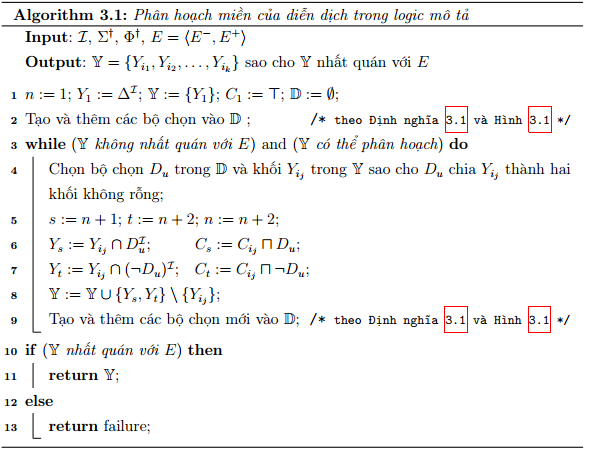
\includegraphics[scale=0.65]{ThuatToan1.png}
\end{frame}


%--------------------------------------------------------------------------
\begin{frame}\frametitle{\bf Học khái niệm cho CSTT với Ngữ cảnh (2)}
	\vspace{-1.5ex}
	\begin{block}{\bf Ngữ cảnh~(2)}
		Bài toán học khái niệm cho cơ sở tri thức trong logic mô tả đặt ra trong ngữ cảnh~(2) là học khái niệm $C$ như là một định nghĩa của $A_d$ trong ngôn ngữ con cho trước $\mLSPD$, với $\SigmaDag \subseteq \Sigma \setminus \{A_d\}$ và $\PhiDag \subseteq \Phi$ sao cho:
		
		\begin{itemize}
			\setlength{\itemsep}{1.0ex}
			\item $\KB \models C(a)$ với mọi $a \in E^+$, và
			\item $\KB \not\models C(a)$, với mọi $a \in E^-$,
		\end{itemize}
		trong đó, tập $E^+$ chứa các mẫu dương và $E^-$ chứa các mẫu âm của $C$.
	\end{block}
	\vspace{-1.0ex}		
	\begin{itemize}
		\setlength{\itemsep}{1.0ex}
		\item Sử dụng các mô hình của $\KB$ kết hợp với mô phỏng hai chiều trong mô hình đó $\rightarrow$ để mô hình hóa tính không phân biệt được.
		
		\item Sử dụng cây quyết định $\rightarrow$ để phân lớp dữ liệu phục vụ cho việc tìm kiếm khái niệm $C$. 
	\end{itemize}
	\vspace{-0.5ex}
	Sử dụng các bộ chọn để làm mịn phân hoạch $\{\Delta^\mI\}$ của diễn dịch $\mI$ là mô hình của $\KB$ nhằm đạt được phân hoạch nhất quán với $E$.
	
\end{frame}

%--------------------------------------------------------------------------
\begin{frame}\frametitle{\bf Ngữ cảnh (2)-Ý tưởng chính của thuật toán \BBCLearnS}
	\vspace{-1.0ex}
	\begin{itemize}
		\setlength{\itemsep}{0.5ex}	
		
		\item Xây dựng tập $E^-_0$ và mở rộng nó sao cho $E^-_0$ phủ càng lúc càng nhiều các cá thể trong $E^-$,
				
		\item Xây dựng tập $\mbC$ gồm các phần tử là các khái niệm $D$ thỏa mãn điều kiện \mbox{$\KB \models D(a)$} với mọi $a \in E^+$.
		
		\item Xây dựng tập $\mbC_0$: khi một khái niệm $D$ không thỏa mãn điều kiện $\KB \models D(a)$ với mọi $a \in E^+$ $\rightarrow$ $D$ được thêm vào $\mbC_0$. Sau này, khi cần, lấy hợp của các khái niệm trong $\mbC_0$ và kiểm tra xem nó có thỏa mãn điều kiện để thêm vào $\mbC$ hay không.
	\end{itemize}
	$\Rightarrow$ Như vậy ta luôn có: 
	\begin{itemize}
		\item $\KB \models (\bigsqcap\mbC)(a)$ $\V a \in E^+$, và
		\item $\KB \not\models (\bigsqcap\mbC)(a)$ $\V a \in E^-_0$.
	\end{itemize}
	\vspace{1.0ex}
	\textcolor{red}{Mở rộng $\mbC$ sao cho $\KB \not\models(\bigsqcap\mbC)(a)$ với càng lúc càng nhiều $a \in E^-$. Mở rộng $\mbC$ $\rightarrow$ mở rộng $E^-_0$. Khi $E^-_0 = E^-$ thuật toán trả về khái niệm $\bigsqcap\mbC$.
		}
\end{frame}

%--------------------------------------------------------------------------
\begin{frame}\frametitle{}
	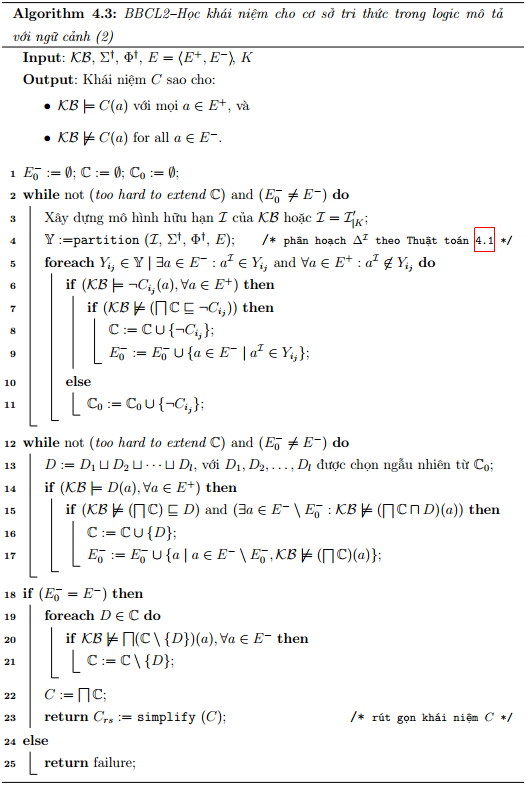
\includegraphics[scale=0.44]{ThuatToan4.png}
\end{frame}

%--------------------------------------------------------------------------
\begin{frame}\frametitle{\bf Tính đúng và độ phức tạp}
	\vspace{-1.5ex}
	\begin{block}{Mệnh đề 3.1 (Tính đúng đắn của thuật toán \BBCLearnS)}
		Thuật toán \BBCLearnS là đúng đắn. Nghĩa là, nếu thuật toán \BBCLearnS trả về một khái niệm $C_{rs}$ thì $C_{rs}$ là một lời giải của bài toán học khái niệm cho cơ sở tri thức trong logic mô tả với ngữ cảnh~(2).\myend
	\end{block}
	\vspace{-1.0ex}
		
	\begin{block}{\bf Độ phức tạp của thuật toán \BBCLearnS}
		Học khái niệm cho cơ sở tri thức trong logic mô tả với ngữ cảnh~(2) liên quan chặt chẽ với suy luận tự động trong logic mô tả. Đối với vấn đề suy luận tự động, độ phức tạp của bài toán này là \EXPTIME-\textnormal{khó} ngay cả đối với logic mô tả cơ bản \ALC. Một cách tổng quát, bài toán kiểm tra tính thỏa trong logic mô tả thường là \EXPTIME-\textnormal{đầy đủ}. Thuật toán \BBCLearn và \BBCLearnS sử dụng một vòng lặp tuyến tính có giới hạn là lực lượng của $\mbC_0$ cho bài toán suy luận. Do đó, hai thuật toán này có độ phức tạp là hàm mũ (xét theo kích thước của $\KB$, $E^+$ và $E^-$ với giả thiết là $\SigmaDag$ cố định).\myend
	\end{block}
\end{frame}

%%--------------------------------------------------------------------------
%\begin{frame}\frametitle{\bf Ví dụ - Thuật toán \BBCLearnS}
%	\vspace{-1.5ex}
%	{\small
%		$\KB'_0 = \tuple{\mR,\mT,\mA'_0}$ như đã cho trong ví dụ~trên và $E = \tuple{E^+, E^-}$, $\SigmaDag$, $\PhiDag$ ($E^+ = \{\Pub_4, \Pub_6\}$, $E^- = \{\Pub_1, \Pub_2, \Pub_3, \Pub_5\}$, $\SigmaDag = \{\Awarded, \Citedby\}$ và $\PhiDag = \emptyset$). Đặt $\KB = \tuple{\mR, \mT, \mA}$ với $\mA = \mA'_0 \cup \{A_d(a) \mid a \in E^+\} \cup \{\neg A_d(a) \mid a \in E^-\}$. 
%		
%		$\mA'_0$ thay cho $\mA_0$ và thuật toán \BBCLearnS thay cho \BBCLearn. Thuật toán \BBCLearnS thực hiện ba bước đầu tiên giống như ví dụ~trên (có bổ sung thêm $E^-_0 := \emptyset$) và các bước tiếp theo như sau:
%		\begin{enumerate}
%			\setcounter{enumi}{3}
%			\item Vì $Y_3 \subseteq E^-$ nên ta tiến hành xem xét đối với $C_3 \equiv \neg\Awarded$. Vì $\KB \models \neg C_3(a)$ với mọi $a \in E^+$ nên ta thêm $\neg C_3$ vào $\mbC$ và thêm các phần tử của $Y_3$ vào $E^-_0$. Do đó, ta có $\mbC = \{C_3\}$ và $E^-_0 = \{\Pub_2,\Pub_3,\Pub_5\}$.
%			
%			\item Vì $Y_5 \subseteq E^-$ nên ta tiến hành xem xét đối với $C_5 \equiv \Awarded \mand \neg\E\Citedby.\top$. Vì $\KB \models \neg C_5(a)$ với mọi $a \in E^+$ và $\bigsqcap\mbC$ không bị bao hàm bởi $C_5$ dựa trên $\KB$ nên ta thêm $\neg C_5$ vào $\mbC$. Do đó, ta có $\mbC = \{\neg C_3, \neg C_5\}$ và $E^-_0 = \{\Pub_1,\Pub_2,\Pub_3,\Pub_5\}$.
%			
%			\item Vì $E^-_0 = E^-$ nên ta có $C \equiv \bigsqcap\mbC \equiv \neg\neg\Awarded \mand \neg(\Awarded \mand \neg \E\Citedby.\top)$. Rút gọn $C$ ta được kết quả trả về là $C_{rs} \equiv \Awarded \mand \E\Citedby.\top$.
%		\end{enumerate}
%	}
%\end{frame}
%
%%--------------------------------------------------------------------------
%\begin{frame}\frametitle{\textbf{Kết quả thực nghiệm}}
%	\vspace{-2.0ex}
%	\begin{itemize}
%		\item Tập dữ liệu \textbf{WebKB}: Web của 4 khoa Khoa học Máy tính
%		
%		\begin{itemize}
%			\item 877 trang web (đối tượng) 
%			\item 1608 liên kết giữa các trang Web của 1 mối quan hệ.
%			\item 5 lớp \texttt{course}, \texttt{faculty}, \texttt{student}, \texttt{project} và \texttt{staff}.
%			\item Dữ liệu huấn luyện: 230 đối tượng và chứng thực: 195 đối tượng. 
%			\item Dữ liệu kiểm tra: 452 đối tượng.
%		\end{itemize} 
%		%--------------------------------------------------------
%		\item Tập dữ liệu \textbf{Family}: British Royal, Bush, Roberts, Romanov, Stevens\!\!\!\!\!\!\!
%		\begin{itemize}
%			\item 943 người (đối tượng) và 11062 liên kết của 6 mối quan hệ.
%			\item Các khái niệm $Male$, $Female$. 
%			\item Dữ liệu huấn luyện: 437 và  chứng thực: 49 đối tượng.
%			\item Dữ liệu kiểm tra: 457 đối tượng.
%		\end{itemize} 
%		
%		\item Tập dữ liệu \textbf{PockerHand}: UCI Machine Learning Repository. 
%		\begin{itemize}
%			\item 2542 tay bài, 12710 quân bài, 119 tính chất (15371 đối tượng) 
%			\item 65220 liên kết của 6 mối quan hệ.
%			\item 6 lớp ``\texttt{one pair}'', ``\texttt{two pairs}'', ``\texttt{three of a~kind}'', ``\texttt{straight}'', ``\texttt{flush}'', ``\texttt{full house}''.   
%			\item Dữ liệu huấn luyện: 1343 đối tượng và chứng thực: 1343 đối tượng. 
%			\item Dữ liệu kiểm tra 12685 đối tượng.
%		\end{itemize}
%	\end{itemize}
%\end{frame}
%%--------------------------------------------------------------------------
%\begin{frame}\frametitle{\textbf{Kết quả thực nghiệm}}
%	Tập dữ liệu WebKB, PockerHand và Family với 100 khái niệm ngẫu nhiên trong logic mô tả~\ALCIQ.
%	\vspace{-2.0ex}
%	{\scriptsize
%		\begin{table}[h!]
%			\centering
%			\begin{tabular}{|l|c|c|c|c|c|c|}
%				\hline
%				\hline
%				\multirow{2}{*}{} &
%				\textbf{\!\!\!Avg. Dep.\!\!\!} & \textbf{\!\!Avg. Len.\!\!} & \textbf{\!\!Avg. Acc.\!\!} & \textbf{\!\!Avg. Pre.\!\!} & \textbf{\!\!Avg. Rec.\!\!} & \textbf{\!\!Avg. F1\!\!}\\
%				& \textbf{\!\!\!Res./Org.\!\!\!} & \textbf{\!\!Res./Org.\!\!} & \textbf{\!\![Min;Max]\!\!} & \textbf{\!\![Min;Max]\!\!} & \textbf{\!\![Min;Max]\!\!} & \textbf{\!\![Min;Max]\!\!}\\
%				%
%				\hline
%				\multicolumn{7}{|l|}{\!\!\textbf{Tập dữ liệu WebKB}}\\
%				\hline  
%				\multirow{2}{*}{\!\!Bộ chọn cơ bản} &\multirow{2}{*}{\!\!\!\!0.82/1.02\!\!\!\!}& \multirow{2}{*}{\!\!\!\!6.81/4.41\!\!\!\!} & \!\!\!\!93.84$\pm$13.50\!\!\!\! & \!\!\!\!92.09$\pm$17.04\!\!\!\! & \!\!\!\!92.82$\pm$17.32\!\!\!\! & \!\!\!\!91.59$\pm$16.68\!\!\!\!\\
%				&  &  & \!\!\!\![33.69;100.0]\!\!\!\! & \!\!\!\![32.08;100.0]\!\!\!\! & \!\!\!\![23.08;100.0]\!\!\!\! & \!\!\!\![27.69;100.0]\!\!\!\!\\
%				\hline
%				\!\!Bộ chọn cơ bản&\multirow{2}{*}{\!\!\!\!0.84/1.02\!\!\!\!}& \multirow{2}{*}{\!\!\!\!3.40/4.41\!\!\!\!}& \!\!\!\!94.60$\pm$12.20\!\!\!\! & \!\!\!\!92.81$\pm$15.93\!\!\!\! & \!\!\!\!93.14$\pm$17.17\!\!\!\! & \!\!\!\!92.33$\pm$16.17\!\!\!\!\\
%				\!\!và mở rộng\!\!\!\! &  &  & \!\!\!\![33.69;100.0]\!\!\!\! & \!\!\!\![32.08;100.0]\!\!\!\! & \!\!\!\![23.08;100.0]\!\!\!\! & \!\!\!\![27.69;100.0]\!\!\!\!\\
%				\hline
%				%
%				\hline
%				\multicolumn{7}{|l|}{\!\!\textbf{Tập dữ liệu PockerHand}}\\
%				\hline
%				\multirow{2}{*}{\!\!Bộ chọn cơ bản} &\multirow{2}{*}{\!\!\!\!1.41/2.60\!\!\!\!}& \multirow{2}{*}{\!\!\!\!37.02/15.97\!\!\!\!} & \!\!\!\!97.17$\pm$08.61\!\!\!\! & \!\!\!\!95.96$\pm$14.99\!\!\!\! & \!\!\!\!94.95$\pm$14.40\!\!\!\! & \!\!\!\!94.66$\pm$14.64\!\!\!\!\\
%				&  &  &\!\!\!\![50.57;100.0]\!\!\!\! & \!\!\!\![01.67;100.0]\!\!\!\! & \!\!\!\![01.67;100.0]\!\!\!\! & \!\!\!\![1.67;100.0]\!\!\!\!\\
%				\hline
%				\!\!Bộ chọn cơ bản&\multirow{2}{*}{1.23/2.60}& \multirow{2}{*}{\!\!\!\!3.47/15.97\!\!\!\!}& \!\!\!\!99.44$\pm$02.15\!\!\!\! & \!\!\!\!98.68$\pm$09.08\!\!\!\! & \!\!\!\!98.06$\pm$09.58\!\!\!\! & \!\!\!\!98.18$\pm$09.14\!\!\!\!\\
%				\!\!và mở rộng\!\!\!\! &  &  & \!\!\!\![83.25;100.0]\!\!\!\! & \!\!\!\![01.67;100.0]\!\!\!\! & \!\!\!\![01.67;100.0]\!\!\!\! & \!\!\!\![1.67;100.0]\!\!\!\!\\
%				\hline
%				%
%				\hline
%				\multicolumn{7}{|l|}{\!\!\textbf{Tập dữ liệu Family}}\\
%				\hline
%				\multirow{2}{*}{\!\!Bộ chọn cơ bản} &\multirow{2}{*}{\!\!\!\!2.38/3.34\!\!\!\!}& \multirow{2}{*}{\!\!\!\!78.50/18.59\!\!\!\!}& \!\!\!\!88.50$\pm$16.65\!\!\!\! & \!\!\!\!90.60$\pm$18.57\!\!\!\! & \!\!\!\!85.66$\pm$22.36\!\!\!\! & \!\!\!\!86.09$\pm$20.10\!\!\!\!\\
%				&  &  & \!\!\!\![27.91;100.0]\!\!\!\! & \!\!\!\![04.55;100.0]\!\!\!\! & \!\!\!\![07.69;100.0]\!\!\!\! & \!\!\!\![08.70;100.0]\!\!\!\!\\
%				\hline
%				\!\!Bộ chọn cơ bản &\multirow{2}{*}{\!\!\!\!2.29/3.34\!\!\!\!}& \multirow{2}{*}{\!\!\!\!10.20/18.59\!\!\!\!}& \!\!\!\!92.79$\pm$14.35\!\!\!\! & \!\!\!\!91.99$\pm$18.40\!\!\!\! & \!\!\!\!91.75$\pm$19.82\!\!\!\! & \!\!\!\!90.39$\pm$19.89\!\!\!\!\\
%				\!\!và mở rộng\!\!\!\! &  &  & \!\!\!\![27.91;100.0]\!\!\!\! & \!\!\!\![04.55;100.0]\!\!\!\! & \!\!\!\![07.69;100.0]\!\!\!\! & \!\!\!\![08.70;100.0]\!\!\!\!\\
%				\hline
%			\end{tabular}
%		\end{table}
%	}
%\end{frame}
%%--------------------------------------------------------------------------
%\begin{frame}\frametitle{\textbf{Kết quả thực nghiệm}}
%	Tập dữ liệu Family với 5 khái niệm trong logic mô tả~\ALCI.
%	{\scriptsize
%		\begin{table}
%			\begin{tabular}{|l | c | c | c | c | c | c |}
%				\hline
%				\hline
%				\multirow{2}{*}{} &
%				\textbf{\!\!\!\!\!Dep.\!\!\!\!\!} & 
%				\textbf{\!\!\!\!\!Len.\!\!\!\!\!} & \textbf{\!\!\!\!\!Avg. Acc.\!\!\!\!\!} & \textbf{\!\!\!\!\!Avg. Pre.\!\!\!\!\!} & \textbf{\!\!\!\!\!Avg. Rec.\!\!\!\!\!} & \textbf{\!\!\!\!\!Avg. F1\!\!\!\!\!}\\
%				& \textbf{\!\!\!\!\!Res.\!\!\!\!\!} & \textbf{\!\!\!\!\!Res.\!\!\!\!\!} & \textbf{\!\!\!\!\!\![Min;Max]\!\!\!\!\!\!} & \textbf{\!\!\!\!\!\![Min;Max]\!\!\!\!\!\!} & \textbf{\!\!\!\!\!\![Min;Max]\!\!\!\!\!\!} & \textbf{\!\!\!\!\!\![Min;Max]\!\!\!\!\!\!}\\
%				%
%				\hline
%				\multicolumn{7}{|l|}{\!\!\textbf{Khái niệm $Grandparent \equiv \E hasChild.(\E hasChild.\top)$}}\\
%				\hline  
%				\multirow{2}{*}{\!\!Bộ chọn cơ bản} &\multirow{2}{*}{2.00}& \multirow{2}{*}{\!\!\!4.00\!\!\!}& \!\!\!100.0$\pm$00.00\!\!\!& \!\!\!100.0$\pm$00.00\!\!\!& \!\!\!100.0$\pm$00.00\!\!\!& \!\!\!100.0$\pm$00.00\!\!\!\\
%				&  &  &\!\!\!\!\!\![100.0;100.0]\!\!\!\!\!\! &\!\!\!\!\!\![100.0;100.0]\!\!\!\!\!\! &\!\!\!\!\!\![100.0;100.0]\!\!\!\!\!\! & \!\!\!\!\!\![100.0;100.0]\!\!\!\!\!\!\\
%				\hline
%				\!\!Bộ chọn cơ bản &\multirow{2}{*}{2.00}& \multirow{2}{*}{4.00}& \!\!\!100.0$\pm$00.00\!\!\!& \!\!\!100.0$\pm$00.00\!\!\!& \!\!\!100.0$\pm$00.00\!\!\!& \!\!\!100.0$\pm$00.00\!\!\!\\
%				\!\!và mở rộng &  &  &\!\!\!\!\!\![100.0;100.0]\!\!\!\!\!\! &\!\!\!\!\!\![100.0;100.0]\!\!\!\!\!\! &\!\!\!\!\!\![100.0;100.0]\!\!\!\!\!\! & \!\!\!\!\!\![100.0;100.0]\!\!\!\!\!\!\\
%				\hline
%				%
%				\hline
%				\multicolumn{7}{| l |}{\!\!\textbf{Khái niệm $Grandfather \equiv Male \mand \E hasChild.(\E hasChild.\top)$}}\\
%				\hline
%				\multirow{2}{*}{\!\!Bộ chọn cơ bản} & \multirow{2}{*}{2.00}& \multirow{2}{*}{36.00}& \!\!\!95.90$\pm$01.39\!\!\!& \!\!\!87.38$\pm$06.81\!\!\!& \!\!\!79.15$\pm$17.38\!\!\!& \!\!\!81.44$\pm$08.35\!\!\!\\
%				&  &  &\!\!\!\!\!\![94.28;97.67]\!\!\!\!\!\! &\!\!\!\!\!\![80.00;96.43]\!\!\!\!\!\! &\!\!\!\!\!\![57.45;100.0]\!\!\!\!\!\! & \!\!\!\!\!\![72.00;92.31]\!\!\!\!\!\!\\
%				\hline
%				\!\!Bộ chọn cơ bản &\multirow{2}{*}{2.00}& \multirow{2}{*}{07.00}& \!\!\!99.46$\pm$00.77\!\!\! & \!\!\!100.0$\pm$00.00\!\!\! & \!\!\!95.74$\pm$6.02\!\!\! & \!\!\!97.73$\pm$03.21\!\!\!\\
%				\!\!và mở rộng &  &  &\!\!\!\!\!\![98.37;100.0]\!\!\!\!\!\! &\!\!\!\!\!\![100.0;100.0]\!\!\!\!\!\! &\!\!\!\!\!\![87.23;100.0]\!\!\!\!\!\! & \!\!\!\!\!\![93.18;100.0]\!\!\!\!\!\!\\
%				\hline
%				%
%				\hline
%				\multicolumn{7}{| l |}{\!\!\textbf{Khái niệm $Grandmother \equiv Female \mand \E hasChild.(\E hasChild.\top)$}} \\
%				\hline
%				\hline
%				\multirow{2}{*}{\!\!Bộ chọn cơ bản} & \multirow{2}{*}{2.00}& \multirow{2}{*}{18.00}& \!\!\!89.74$\pm$01.30\!\!\!& \!\!\!100.0$\pm$00.00\!\!\!& \!\!\!15.32$\pm$04.47\!\!\!& \!\!\!26.31$\pm$06.85\!\!\!\\
%				&  &  &\!\!\!\!\!\![88.37;91.49]\!\!\!\!\!\! &\!\!\!\!\!\![100.0;100.0]\!\!\!\!\!\! &\!\!\!\!\!\![09.30;20.00]\!\!\!\!\!\! & \!\!\!\!\!\![17.02;33.33]\!\!\!\!\!\!\\
%				\hline
%				\!\!Bộ chọn cơ bản &\multirow{2}{*}{2.00}& \multirow{2}{*}{07.00}& \!\!\!99.91$\pm$00.13\!\!\! & \!\!\!100.0$\pm$00.00\!\!\! & \!\!\!99.22$\pm$01.10\!\!\! & \!\!\!99.61$\pm$00.55\!\!\!\\
%				\!\!và mở rộng &  &  &\!\!\!\!\!\![99.73;100.0]\!\!\!\!\!\! &\!\!\!\!\!\![100.0;100.0]\!\!\!\!\!\! &\!\!\!\!\!\![97.67;100.0]\!\!\!\!\!\! & \!\!\!\!\!\![98.82;100.0]\!\!\!\!\!\!\\
%				\hline
%				\hline
%			\end{tabular}
%		\end{table}
%	}
%\end{frame}
%%--------------------------------------------------------------------------
%\begin{frame}\frametitle{\textbf{Kết quả thực nghiệm}}
%	Tập dữ liệu Family với 5 khái niệm trong logic mô tả~\ALCI.
%	{\scriptsize
%		\begin{table}
%			\begin{tabular}{|l | c | c | c | c | c | c |}
%				\hline
%				\hline
%				\multirow{2}{*}{} &
%				\textbf{\!\!\!\!\!Dep.\!\!\!\!\!} & 
%				\textbf{\!\!\!\!\!Len.\!\!\!\!\!} & \textbf{\!\!\!\!\!Avg. Acc.\!\!\!\!\!} & \textbf{\!\!\!\!\!Avg. Pre.\!\!\!\!\!} & \textbf{\!\!\!\!\!Avg. Rec.\!\!\!\!\!} & \textbf{\!\!\!\!\!Avg. F1\!\!\!\!\!}\\
%				& \textbf{\!\!\!\!\!Res.\!\!\!\!\!} & \textbf{\!\!\!\!\!Res.\!\!\!\!\!} & \textbf{\!\!\!\!\!\![Min;Max]\!\!\!\!\!\!} & \textbf{\!\!\!\!\!\![Min;Max]\!\!\!\!\!\!} & \textbf{\!\!\!\!\!\![Min;Max]\!\!\!\!\!\!} & \textbf{\!\!\!\!\!\![Min;Max]\!\!\!\!\!\!}\\
%				%
%				\hline
%				\hline
%				\multicolumn{7}{| l |}{\!\!\textbf{Khái niệm $Niece \equiv Female \mand \E hasChild^-.(\E hasBrother.\top \mor \E hasSister.\top)$}} \\
%				\hline
%				\multirow{2}{*}{\!\!Bộ chọn cơ bản} &\multirow{2}{*}{3.00}&
%				\multirow{2}{*}{151.00}& \!\!\!85.57$\pm$09.47\!\!\! & \!\!\!57.92$\pm$32.09\!\!\! & \!\!\!64.70$\pm$29.35\!\!\! & \!\!\!60.69$\pm$31.33\!\!\!\\
%				&  &  &\!\!\!\!\!\![72.21;93.02]\!\!\!\!\!\! & \!\!\!\!\!\![12.66;83.33]\!\!\!\!\!\! & \!\!\!\!\!\![23.26;87.50]\!\!\!\!\!\! & \!\!\!\!\!\![16.39;83.33]\!\!\!\!\!\!\\
%				\hline
%				\!\!Bộ chọn cơ bản &\multirow{2}{*}{2.00}& \multirow{2}{*}{11.00}& \!\!\!100.0$\pm$00.00\!\!\! & \!\!\!100.0$\pm$00.00\!\!\! & \!\!\!100.0$\pm$00.00\!\!\! & \!\!\!100.0$\pm$00.00\!\!\!\\
%				\!\!và mở rộng &  &  &\!\!\!\!\!\![100.0;100.0]\!\!\!\!\!\! &\!\!\!\!\!\![100.0;100.0]\!\!\!\!\!\! &\!\!\!\!\!\![100.0;100.0]\!\!\!\!\!\! & \!\!\!\!\!\![100.0;100.0]\!\!\!\!\!\!\\
%				\hline
%				\hline
%				\multicolumn{7}{| l |}{\!\!\textbf{Khái niệm $Nephew \equiv Male \mand \E hasChild^-.(\E hasBrother.\top \mor \E hasSister.\top)$}} \\
%				\hline
%				\multirow{2}{*}{\!\!Bộ chọn cơ bản} &\multirow{2}{*}{3.00}&
%				\multirow{2}{*}{178.00}& \!\!\!91.40$\pm$05.74\!\!\! & \!\!\!77.04$\pm$26.30\!\!\! & \!\!\!88.40$\pm$01.99\!\!\! & \!\!\!79.82$\pm$17.72\!\!\!\\
%				&  &  &\!\!\!\!\!\![83.38;95.74]\!\!\!\!\!\! &\!\!\!\!\!\![40.22;100.0]\!\!\!\!\!\! &\!\!\!\!\!\![86.05;90.91]\!\!\!\!\!\! & \!\!\!\!\!\![54.81;93.75]\!\!\!\!\!\!\\
%				\hline
%				\!\!Bộ chọn cơ bản &\multirow{2}{*}{2.00}& \multirow{2}{*}{11.00}& \!\!\!100.0$\pm$00.00\!\!\! & \!\!\!100.0$\pm$00.00\!\!\! & \!\!\!100.0$\pm$00.00\!\!\! & \!\!\!100.0$\pm$00.00\!\!\!\\
%				\!\!và mở rộng &  &  &\!\!\!\!\!\![100.0;100.0]\!\!\!\!\!\! &\!\!\!\!\!\![100.0;100.0]\!\!\!\!\!\! &\!\!\!\!\!\![100.0;100.0]\!\!\!\!\!\! & \!\!\!\!\!\![100.0;100.0]\!\!\!\!\!\!\\
%				\hline    
%			\end{tabular}
%		\end{table}
%	}
%\end{frame}
%%--------------------------------------------------------------------------
%\begin{frame}\frametitle{\textbf{Kết quả thực nghiệm}}
%	Tập dữ liệu Pocker Hand với 6 tập đối tượng trong logic mô tả~\ALCQ.
%	{\scriptsize
%		\begin{table}
%			\begin{tabular}{|l | c | c | c | c | c | c |}
%				\hline
%				\hline
%				\multirow{2}{*}{} & \textbf{\!\!\!Dep.\!\!\!} & \textbf{\!\!Len.\!\!} & \textbf{\!\!\!Avg. Acc.\!\!\!} & \textbf{\!\!\!Avg. Pre.\!\!\!} & \textbf{\!\!\!Avg. Rec.\!\!\!} & \textbf{\!\!\!Avg. F1\!\!\!}\\
%				& \textbf{\!\!\!Res.\!\!\!} & \textbf{\!\!Res.\!\!} & \textbf{\!\!\!\![Min;Max]\!\!\!\!} & \textbf{\!\!\!\![Min;Max]\!\!\!\!} & \textbf{\!\!\!\![Min;Max]\!\!\!\!} & \textbf{\!\!\!\![Min;Max]\!\!\!\!}\\
%				%
%				\hline
%				\multicolumn{7}{|l|}{\!\!\textbf{Tập ``\texttt{one pair}''}}\\
%				\hline  
%				\multirow{2}{*}{\!\!Bộ chọn cơ bản} &\multirow{2}{*}{4.0}& \multirow{2}{*}{109.00}& \!\!\!42.57$\pm$01.48\!\!\!& \!\!\!16.74$\pm$00.87\!\!\!& \!\!\!76.00$\pm$4.03\!\!\!& \!\!\!27.44$\pm$01.42\!\!\!\\
%				&  &  &\!\!\!\![40.71;45.24]\!\!\!\! &\!\!\!\![15.64;18.05]\!\!\!\! &\!\!\!\![71.67;81.67]\!\!\!\! & \!\!\!\![25.67;29.45]\!\!\!\!\\
%				\hline
%				\!\!Bộ chọn cơ bản&\multirow{2}{*}{5.00}& \multirow{2}{*}{15.00}& \!\!\!100.0$\pm$00.00\!\!\!& \!\!\!100.0$\pm$00.00\!\!\!& \!\!\!100.0$\pm$00.00\!\!\!& \!\!\!100.0$\pm$00.00\!\!\!\\
%				\!\!và mở rộng &  &  &\!\!\!\![100.0;100.0]\!\!\!\! &\!\!\!\![100.0;100.0]\!\!\!\! &\!\!\!\![100.0;100.0]\!\!\!\! & \!\!\!\![100.0;100.0]\!\!\!\!\\
%				\hline
%				%
%				\hline
%				\multicolumn{7}{|l|}{\!\!\textbf{Tập ``\texttt{two pairs}''}}\\
%				\hline
%				\multirow{2}{*}{\!\!Bộ chọn cơ bản} &\multirow{2}{*}{4.00}&
%				\multirow{2}{*}{25.00}& \!\!\!36.33$\pm$00.47\!\!\! & \!\!\!17.16$\pm$0.53\!\!\! & \!\!\!90.33$\pm$4.14\!\!\! & \!\!\!28.83$\pm$00.96\!\!\!\\
%				&  &  &\!\!\!\![35.48;36.67]\!\!\!\! &\!\!\!\![16.34;17.70]\!\!\!\! &\!\!\!\![83.33;95.00]\!\!\!\! & \!\!\!\![27.32;29.84]\!\!\!\!\\
%				\hline
%				\!\!Bộ chọn cơ bản&\multirow{2}{*}{5.00}& \multirow{2}{*}{15.00}& \!\!\!100.0$\pm$00.00\!\!\!& \!\!\!100.0$\pm$00.00\!\!\!& \!\!\!100.0$\pm$00.00\!\!\!& \!\!\!100.0$\pm$00.00\!\!\!\\
%				\!\!và mở rộng &  &  &\!\!\!\![100.0;100.0]\!\!\!\! &\!\!\!\![100.0;100.0]\!\!\!\! &\!\!\!\![100.0;100.0]\!\!\!\! & \!\!\!\![100.0;100.0]\!\!\!\!\\
%				\hline
%				%
%				\hline
%				\multicolumn{7}{|l|}{\!\!\textbf{Tập ``\texttt{three of a~kind}''}} \\
%				\hline
%				\multirow{2}{*}{\!\!Bộ chọn cơ bản} &\multirow{2}{*}{4.00}&
%				\multirow{2}{*}{48.00}& \!\!\!52.52$\pm$02.16\!\!\! & \!\!\!20.92$\pm$1.01\!\!\! & \!\!\!83.33$\pm$01.83\!\!\! & \!\!\!33.43$\pm$01.39\!\!\!\\
%				&  &  &\!\!\!\![50.71;56.67]\!\!\!\! &\!\!\!\![19.75;22.77]\!\!\!\! &\!\!\!\![80.00;85.00]\!\!\!\! & \!\!\!\![31.68;35.92]\!\!\!\!\\
%				\hline
%				\!\!Bộ chọn cơ bản&\multirow{2}{*}{3.00}& \multirow{2}{*}{11.00}& \!\!\!100.0$\pm$00.00\!\!\!& \!\!\!100.0$\pm$00.00\!\!\!& \!\!\!100.0$\pm$00.00\!\!\!& \!\!\!100.0$\pm$00.00\!\!\!\\
%				\!\!và mở rộng &  &  &\!\!\!\![100.0;100.0]\!\!\!\! &\!\!\!\![100.0;100.0]\!\!\!\! &\!\!\!\![100.0;100.0]\!\!\!\! & \!\!\!\![100.0;100.0]\!\!\!\!\\
%				\hline
%			\end{tabular}
%		\end{table}
%	}
%\end{frame}
%%--------------------------------------------------------------------------
%\begin{frame}\frametitle{\textbf{Kết quả thực nghiệm}}
%	Tập dữ liệu Pocker Hand với 6 tập đối tượng trong logic mô tả~\ALCQ.
%	{\scriptsize
%		\begin{table}
%			\begin{tabular}{|l | c | c | c | c | c | c |}
%				\hline
%				\hline
%				\multirow{2}{*}{} & \textbf{\!\!\!Dep.\!\!\!} & \textbf{\!\!Len.\!\!} & \textbf{\!\!\!Avg. Acc.\!\!\!} & \textbf{\!\!\!Avg. Pre.\!\!\!} & \textbf{\!\!\!Avg. Rec.\!\!\!} & \textbf{\!\!\!Avg. F1\!\!\!}\\
%				& \textbf{\!\!\!Res.\!\!\!} & \textbf{\!\!Res.\!\!} & \textbf{\!\!\!\![Min;Max]\!\!\!\!} & \textbf{\!\!\!\![Min;Max]\!\!\!\!} & \textbf{\!\!\!\![Min;Max]\!\!\!\!} & \textbf{\!\!\!\![Min;Max]\!\!\!\!}\\
%				%
%				\hline
%				\multicolumn{7}{|l|}{\!\!\textbf{Tập ``\texttt{straight}''}} \\
%				\hline
%				\multirow{2}{*}{\!\!Bộ chọn cơ bản} &\multirow{2}{*}{5.00}&
%				\multirow{2}{*}{97.00}& \!\!\!81.24$\pm$02.01\!\!\! & \!\!\!39.65$\pm$04.62\!\!\! & \!\!\!58.33$\pm$04.94\!\!\! & \!\!\!47.13$\pm$4.41\!\!\!\\
%				&  &  &\!\!\!\![80.00;85.24]\!\!\!\! &\!\!\!\![36.36;48.72]\!\!\!\! &\!\!\!\![53.33;65.00]\!\!\!\! & \!\!\!\![43.24;55.07]\!\!\!\!\\
%				\hline
%				\!\!Bộ chọn cơ bản&\multirow{2}{*}{5.00}& \multirow{2}{*}{32.00}& \!\!\!98.67$\pm$00.68\!\!\! & \!\!\!96.35$\pm$03.44\!\!\! & \!\!\!94.33$\pm$02.00\!\!\! & \!\!\!95.31$\pm$02.35\!\!\!\\
%				\!\!và mở rộng &  &  &\!\!\!\![97.62;99.52]\!\!\!\! &\!\!\!\![90.32;100.0]\!\!\!\! &\!\!\!\![91.67;96.67]\!\!\!\! & \!\!\!\![91.80;98.31]\!\!\!\!\\
%				\hline
%				\hline
%				\multicolumn{7}{|l|}{\!\!\textbf{Tập ``\texttt{flush}''}} \\
%				\hline
%				\multirow{2}{*}{\!\!Bộ chọn cơ bản} &\multirow{2}{*}{2.00}&
%				\multirow{2}{*}{10.00}& \!\!\!94.33$\pm$00.80\!\!\! & \!\!\!71.71$\pm$02.79\!\!\! & \!\!\!100.0$\pm$00.00\!\!\! & \!\!\!83.49$\pm$01.92\!\!\!\\
%				&  &  &\!\!\!\![92.86;95.24]\!\!\!\! &\!\!\!\![66.67;75.00]\!\!\!\! &\!\!\!\![100.0;100.0]\!\!\!\! & \!\!\!\![80.00;85.71]\!\!\!\!\\
%				\hline
%				\!\!Bộ chọn cơ bản&\multirow{2}{*}{3.00}& \multirow{2}{*}{7.00}& \!\!\!100.0$\pm$00.00\!\!\!& \!\!\!100.0$\pm$00.00\!\!\!& \!\!\!100.0$\pm$00.00\!\!\!& \!\!\!100.0$\pm$00.00\!\!\!\\
%				\!\!và mở rộng &  &  &\!\!\!\![100.0;100.0]\!\!\!\! &\!\!\!\![100.0;100.0]\!\!\!\! &\!\!\!\![100.0;100.0]\!\!\!\! & \!\!\!\![100.0;100.0]\!\!\!\!\\
%				\hline
%				\hline
%				\multicolumn{7}{|l|}{\!\!\textbf{Tập ``\texttt{full house}''}} \\
%				\hline
%				\multirow{2}{*}{\!\!Bộ chọn cơ bản} &\multirow{2}{*}{4.00}&
%				\multirow{2}{*}{68.00}& \!\!\!60.48$\pm$03.05\!\!\! & \!\!\!25.95$\pm$01.45\!\!\! & \!\!\!94.67$\pm$2.45\!\!\! & \!\!\!40.71$\pm$01.73\!\!\!\\
%				&  &  &\!\!\!\![57.62;64.76]\!\!\!\! &\!\!\!\![24.23;28.00]\!\!\!\! &\!\!\!\![91.67;98.33]\!\!\!\! & \!\!\!\![38.33;43.08]\!\!\!\!\\
%				\hline
%				\!\!Bộ chọn cơ bản&\multirow{2}{*}{2.00}& \multirow{2}{*}{6.00}& \!\!\!100.0$\pm$00.00\!\!\!& \!\!\!100.0$\pm$00.00\!\!\!& \!\!\!100.0$\pm$00.00\!\!\!& \!\!\!100.0$\pm$00.00\!\!\!\\
%				\!\!và mở rộng &  &  &\!\!\!\![100.0;100.0]\!\!\!\! &\!\!\!\![100.0;100.0]\!\!\!\! &\!\!\!\![100.0;100.0]\!\!\!\! & \!\!\!\![100.0;100.0]\!\!\!\!\\
%				\hline
%			\end{tabular}
%		\end{table}
%	}
%\end{frame}

%--------------------------------------------------------------------------
\begin{frame}\frametitle{\bf Kết quả nghiên cứu của đề}
	\vspace{-1.0ex}
%	{\small
	\begin{enumerate}
		\setlength{\itemsep}{2.0ex}
		\item Xây dựng ngôn ngữ logic mô tả $\mLSP$ dựa trên ngôn ngữ \ALCreg với tập các đặc trưng mở rộng gồm $\mI$, $\mO$, $\mN$, $\mQ$, $\mF$, $\mU$, $\Self$. Ngoài ra ngôn ngữ được xây dựng còn cho phép sử dụng các thuộc tính như là các phần tử cơ bản của ngôn ngữ.
		
		\item Xây dựng mô phỏng hai chiều trên lớp các logic mở rộng. Phát biểu và chứng minh các định lý, bổ đề, hệ quả liên quan đến mô phỏng hai chiều và tính bất biến đối với mô phỏng hai chiều.
		
		\item Xây dựng thuật toán \BBCLearnS nhằm giải quyết các bài toán học khái niệm cho cơ sở tri thức trong logic mô tả với ngữ cảnh~(2).
	\end{enumerate}
%	}
\end{frame}
%----------------------------------------------------------------------------------------

\begin{frame}\frametitle{\bf Các vấn đề cần quan tâm nghiên cứu thêm}
	\begin{enumerate}
		\setlength{\itemsep}{1.5ex}
		\item Xây dựng các chiến lược học khác nhau thông qua các độ đo trong việc quyết định khối nào nên phân hoạch trước. So sánh các chiến lược học với nhau.
		
		\item Xây dựng các module học khái niệm trong logic mô tả với các ngữ cảnh khác nhau như là một API cho phép tích hợp vào các hệ thống khác.
		
		\item Nghiên cứu các thuật toán học nữa giám sát, học không giám sát, học theo xác suất cho các cở sở tri thức trong logic mô tả.
		
		\item Nghiên cứu khả năng học chính xác khái niệm cho các logic mô tả khác nhau.
	\end{enumerate}
\end{frame}

%--------------------------------------------------------------------------
\begin{frame}\frametitle{\bf Danh mục các công trình đã công bố}
	
\vspace{-1.0ex}
\begin{scriptsize}
	\begin{enumerate}
		\item Trần Thanh Lương, Hoàng Thị Lan Giao. \textcolor{red}{Áp dụng độ đo entropy để phân hoạch khối cho các hệ thống thông tin dựa trên logic mô tả}. {\em Kỷ yếu Hội thảo quốc gia lần thứ XV: Một số vấn đề chọn lọc của Công nghệ Thông tin và Truyền thông}, trang 11--18, Nhà xuất bản Khoa học và Kỹ thuật, 2013.	
		
		\item T.-L. Tran, Q.-T. Ha, T.-L.-G. Hoang, L. A. Nguyen, and H. S. Nguyen. Bisimulation-based concept learning in description logics. In {\em Proceedings of CS\&P'2013}, pages 421--433. CEURWS.org, 2013.
		
		\item T.-L. Tran, L. A. Nguyen, and T.-L.-G. Hoang. \textcolor{red}{A domain partitioning method for bisimulationbased concept learning in description logics}. In {\em Proceedings of ICCSAMA'2014, volume 282 of Advances in Intelligent Systems and Computing}, pages 297--312. Springer, 2014.
		
		\item T.-L. Tran, Q.-T. Ha, T.-L.-G. Hoang, L. A. Nguyen, and H. S. Nguyen. \textcolor{red}{Bisimulation-based concept learning in description logics}. {\em Fundam. Inform.}, 133(2-3):287--303, 2014.
		
		\item T.-L. Tran, T.-L.-G. Hoang. \textcolor{red}{Entropy-based measures for partitioning the domain of an interpretation in description logics}. {\em Journal of Science, Hue University}, volume 96, number 8: pages 87-101, 2014.
		
		\item T.-L. Tran, L. A. Nguyen, and  T.-L.-G. Hoang. \textcolor{red}{Bisimulation-based concept learning for information systems in description logics}. {\em Vietnam Journal of Computer Science}, Springer, 2015. (Online first).
	\end{enumerate}
\end{scriptsize}
\end{frame}

%--------------------------------------------------------------------------
\begin{frame}\frametitle{\bf Danh mục các sản phẩm đào tạo}
{\bf Đào tạo thạc sĩ}
\begin{small}
	\begin{itemize}
		\item Họ tên: Nguyễn Công Ẩn,\qquad\;Khóa 2011--2013, Chuyên ngành KHMT\\	
		Đề tài: Nghiên cứu một số thuật toán suy luận trong logic mô tả\\	
		Năm thực hiện: 2013\\
		Người hướng dẫn: Hoàng Thị Lan Giao (thành viên đề tài)
	\end{itemize}
\end{small}

{\bf Đào tạo cử nhân}
\begin{small}
	\begin{itemize}
		\item Họ tên: Nguyễn Hữu Hải,\qquad\, Khóa 33, Ngành Tin học\\	
		Đề tài: Tìm hiểu về logic mô tả và ứng dụng trong xây dựng ontology\\	
		Năm thực hiện: 2013\\	
		Người hướng dẫn: Trần Thanh Lương (chủ nhiệm đề tài)
		
		\item Họ tên: Đặng Tuấn Anh,\qquad\;\;\;Khóa 34, Ngành Tin học\\	
		Đề tài: Phân lớp dữ liệu với nhiều tập huấn luyện bằng cây quyết định\\	
		Năm thực hiện: 2014\\	
		Người hướng dẫn: Trần Thanh Lương (chủ nhiệm đề tài)
	\end{itemize}
\end{small}
\end{frame}

%--------------------------------------------------------------------------
\begin{frame}\frametitle{}
	\begin{center}
		\textcolor{blue}{\Large \bf XIN CẢM ƠN QUÝ THẦY CÔ\\[0.5ex]
			VÀ CÁC ANH CHỊ ĐÃ LẮNG NGHE!}
	\end{center}

\end{frame}
\end{document}